\documentclass[a4paper,11pt]{memoir}

\usepackage[utf8]{inputenc}
\usepackage[final]{microtype}
\usepackage{amsmath,amssymb,mathtools}
\usepackage{graphicx}
\usepackage{minted}
\usepackage{comment}
\usepackage{bbm}
\usepackage{multirow}
\usepackage{dsfont}


\usepackage[utf8]{inputenc}
\usepackage[final]{microtype}
\usepackage{amsmath,amssymb,mathtools}
\usepackage{graphicx}

%%% PAGE LAYOUT 
%%%------------------------------------------------------------------------------

\setlrmarginsandblock{0.15\paperwidth}{*}{1} % Left and right margin
\setulmarginsandblock{0.2\paperwidth}{*}{1}  % Upper and lower margin
\checkandfixthelayout

\maxsecnumdepth{subsection} % Subsections (and higher) are numbered
\setsecnumdepth{subsection}
\chapterstyle{reparticle}

\setsecheadstyle{\normalfont\large\bfseries}
\setsubsecheadstyle{\normalfont\normalsize\bfseries}
\setparaheadstyle{\normalfont\normalsize\bfseries}
\setparaindent{0pt}\setafterparaskip{0pt}

\usepackage{xcolor}
\usepackage{listings}
\usepackage{makecell}

\definecolor{codegreen}{rgb}{0,0.6,0}
\definecolor{codegray}{rgb}{0.5,0.5,0.5}
\definecolor{codepurple}{rgb}{0.58,0,0.82}
\definecolor{backcolour}{rgb}{0.95,0.95,0.92}
 
\lstdefinestyle{mystyle}{
    backgroundcolor=\color{backcolour},   
    commentstyle=\color{codegreen},
    keywordstyle=\color{magenta},
    numberstyle=\tiny\color{codegray},
    stringstyle=\color{codepurple},
    basicstyle=\footnotesize,
    breakatwhitespace=false,         
    breaklines=true,                 
    captionpos=b,                    
    keepspaces=true,                 
    numbers=left,                    
    numbersep=5pt,                  
    showspaces=false,                
    showstringspaces=false,
    showtabs=false,                  
    tabsize=2
}
 
\lstset{style=mystyle}

\makeatletter                  % You do not need to write [htpb] all the time
\renewcommand\fps@figure{htbp} %
\renewcommand\fps@table{htbp}  %
\makeatother                   %

\newcommand\function[1]{\textcolor{blue}{\bm\texttt{#1}}}

\captiondelim{\space } % A space between caption name and text
\captionnamefont{\small\bfseries} % Font of the caption name
\captiontitlefont{\small\normalfont} % Font of the caption text

\changecaptionwidth          % Change the width of the caption
\captionwidth{1\textwidth} %

\makepagestyle{standard} % Make standard pagestyle

\makeatletter                 % Define standard pagestyle
\makeevenfoot{standard}{}{}{} %
\makeoddfoot{standard}{}{}{}  %
\makeevenhead{standard}{\bfseries\thepage\normalfont\qquad\small\leftmark}{}{}
\makeoddhead{standard}{}{}{\small\rightmark\qquad\bfseries\thepage}
% \makeheadrule{standard}{\textwidth}{\normalrulethickness}
\makeatother                  %

\makeatletter
\makepsmarks{standard}{
\createmark{chapter}{both}{shownumber}{}{ \quad }
\createmark{section}{right}{shownumber}{}{ \quad }
\createplainmark{toc}{both}{\contentsname}
\createplainmark{lof}{both}{\listfigurename}
\createplainmark{lot}{both}{\listtablename}
\createplainmark{bib}{both}{\bibname}
\createplainmark{index}{both}{\indexname}
\createplainmark{glossary}{both}{\glossaryname}
}
\makeatother                               

\nouppercaseheads
\pagestyle{standard}               % Choosing pagestyle and chapter pagestyle
\aliaspagestyle{chapter}{chap} %

%%% NEW COMMANDS
%%%------------------------------------------------------------------------------

\newcommand{\p}{\partial} %Partial
% Or what ever you want

%%% TABLE OF CONTENTS
%%%------------------------------------------------------------------------------

\maxtocdepth{subsection} % Only parts, chapters and sections in the table of contents
\settocdepth{subsection}

\AtEndDocument{\addtocontents{toc}{\par}} % Add a \par to the end of the TOC

%%% INTERNAL HYPERLINKS
%%%-------------------------------------------------------------------------------

\usepackage{hyperref}   % Internal hyperlinks
\hypersetup{
pdfborder={0 0 0},      % No borders around internal hyperlinks
pdfauthor={I am the Author} % author
}
\usepackage{memhfixc}   %


%%% References
\usepackage[square,numbers]{natbib}
\bibliographystyle{abbrvnat}
\setcitestyle{authoryear,open={((},close={))}} 


\usepackage{subcaption}

\makeatletter
\def\maketitle{%
  \null
  \thispagestyle{empty}%
  \vfill
  \begin{center}\leavevmode
    \normalfont
    {\LARGE\raggedleft \@author\par}%
    \hrulefill\par
    {\huge\raggedright \@title\par}%
    \vskip 1cm
%    {\Large \@date\par}%
  \end{center}%
  \vfill
  \null
  \cleardoublepage
  }
\makeatother
\title{User Manual for Consensus Rankings User Interface}
\date{}

\begin{document}

\let\cleardoublepage\clearpage

\maketitle


\tableofcontents

\clearpage

\chapter{Main interface}
\section{Initialization}

Before downloading the package \texttt{RankingTool}, 
please make sure all dependencies were installed.
The following dependencies are required:
\begin{itemize}
  \item \texttt{PIL, json, os, tkinter, matplotlib}
  \item \texttt{pyautogui, pandas, toml, sys}
  \item \texttt{ry2, subprocess}
\end{itemize}

Download the package using
\begin{lstlisting}[language=Python]
		pip install rankingTool==1.0
\end{lstlisting}


To initialize the GUI, the user needs a configuration file. 
An example of the configuration file is provided in \texttt{config.toml}.
Specifically, it contains the following arguments:
\begin{enumerate}
  \item \textbf{[default]}
  \begin{itemize}
    \item name (str): name of the rankings UI.
    \item num\_str (int): length of strings allowed for the ``short'' version of the item names.
    \item rat\_min (int): minimum of the ratings.
    \item rat\_max (int): maximum of all the ratings.
    \item overall\_merit\_max (int): minimum of the overall ratings.
    \item overall\_merit\_min (int): maximum of the overall ratings.
    \item topk (int): number of top items included.
  \end{itemize}

  \item \textbf{[default\_graphic\_attributes]}
   \begin{itemize}
    \item color (str): default background color of item boxes.
    \item outline (str): default color of the outline of item boxes.
    \item width (int): default width of the outline of item boxes.
    \item dash (int): default dash type of the outline of item boxes.
      \end{itemize}


  \item \textbf{[graphic\_to\_rating]}
   \begin{itemize}
    \item Bands (str): {\color{red} Seems currently useless in codes?}
    \item Box\_Background\_Color (str): feature represented by the background colors of item boxes.
    \item Width (str): feature represented by the width of the outline of item boxes.
    \item Dash (str): feature represented by dash types of the outline of item boxes.
    \item Outline (str): feature represented by colors of the outline of item boxes.
      \end{itemize}


  \item \textbf{[review]}
   \begin{itemize}
    \item titles (str): {feature name of the text review.}
      \end{itemize}

  \item \textbf{[filter]}
   \begin{itemize}
    \item yesno\_list (lst): {\color{red} Seems currently useless in codes?}
      \end{itemize}

  \item \textbf{[box\_size]}
     \begin{itemize}
    \item box\_width (numeric): width of each item box.
    \item box\_height (numeric): height of each item box.
    \item box\_distance\_x  (numeric): distance along x axis between adjacent item boxes.
    \item box\_distance\_y  (numeric): distance along y axis between adjacent item boxes.
    \item ranking\_area\_x  (numeric): total length of the ranking area along x axis.
      \end{itemize}

  \item \textbf{[box\_graph\_attributes]}: 
  this part specifies the values of ratings represented by the graphical attributes.
  {\color{red} Currently using integers.}
  \begin{itemize}
    \item{} [box\_graph\_attributes.color]: rating (numeric) = color (str).
    \item{} [box\_graph\_attributes.width]: rating (numeric) = width (numeric).
    \item{} [box\_graph\_attributes.dash]: rating (numeric) = dash type (tuple).
  \end{itemize}

\end{enumerate}

After installation and preparation of the configuration file, the GUI can be opened by running the \texttt{main.py} file with the following codes:

\begin{lstlisting}[language=Python]
instance = GUI(``config.toml'')
instance.show()
\end{lstlisting}

\begin{comment}
Users might need to preprocess different input files into specific format and pass them into the classes of Rankings, Reviews, Reviewers, and Proposals, and then to pass the four classes and a configuration file into the GUI.

\textbf{Specific Parameter Format for Each Class:}


\begin{lstlisting}[language=Python]
	GUI(rankings, reviewers, reviews, props, configs_path, mactouchpad=True)
\end{lstlisting}

\begin{itemize}
  \item[--] \textbf{rankings:} The Rankings class constructed by using the input files.
  \item[--] \textbf{reviewers:} The Reviewers class constructed by using the input files.
  \item[--] \textbf{reviews:} The Reviews class constructed by using the input files.
  \item[--] \textbf{props:} The Rroposals class constructed by using the input files.
  \item[--] \textbf{configs{\textunderscore}path:} The path of the configuration file.
  \item[--] \textbf{mactouchpad:} The variable indicating if the user is using a macbook touchpad. The default is True. If using a classic mouse, please turn it to False.
\end{itemize}

\begin{lstlisting}[language=Python]
	Rankings(rating_df, ranking, ties, rating_names, reviewer_col_name="Reviewer Name", prop_col_name="Proposal Name", overall_col_name="Overall Score")
\end{lstlisting}
\begin{itemize}
  \item[--] \textbf{rating\textunderscore df:} A pandas dataframe without any index that has columns for every rating, reviewer name, proposal name, and overall merit, and each row contains ratings that a given reviewer gave for a given proposal. 
  \item[--] \textbf{ranking:} A dictionary that the keys are the reviewer names and the values are the list of proposals in the descending ranking order that the reviewer gave.
  \item[--] \textbf{rating\textunderscore names:} A list of rating names.
  \item[--] \textbf{reviewer\textunderscore col\textunderscore name:} The column name of the reviewer names that the users gave in the dataframe of rating\textunderscore df. The default is "Reviewer Name".
  \item[--] \textbf{prop\textunderscore col\textunderscore name:} The column name of the proposal names that the users gave in the dataframe of rating\textunderscore df. The default is "Proposal Name".
  \item[--] \textbf{reviewer\textunderscore col\textunderscore name:} The column name of the overall merit that the users gave in the dataframe of rating\textunderscore df. The default is "Overall Score".
\end{itemize}

\begin{lstlisting}[language=Python]
	Reviews(df, review_titles, prop_colname="Proposal Name", reviewer_colname="Reviewer Name", str_wrap_len=35)
\end{lstlisting}
\begin{itemize}
  \item[--] \textbf{df:} A dataframe without any index that has columns for every review text, proposal names, reviewers names, and numerical ratings (optional), and each row contains review text of the proposal given by the reviewer.
  \item[--] \textbf{review\textunderscore titles:} A list of column names of each review title in the df above.
  \item[--] \textbf{prop\textunderscore col\textunderscore name:} The column name of the proposal names that the users gave in the dataframe of rating\textunderscore df. The default is "Proposal Name".
  \item[--] \textbf{reviewer\textunderscore{col}\textunderscore{name}:} The column name of the reviewer names that the users gave in the dataframe of rating\textunderscore df. The default is "Reviewer Name".
  \item[--] \textbf{str\textunderscore{wrap}\textunderscore{len}:} A int that indicated the length of string wrapped in the window of review text. The default is 35.
\end{itemize}

\begin{lstlisting}[language=Python]
	Reviewers(df)
\end{lstlisting}

\begin{itemize}
  \item[--] \textbf{df:} The rating\textunderscore df obtained from \texttt{Rankings}.
\end{itemize}

\begin{minted}{python}
	Proposals(df)
\end{minted}
\begin{itemize}
  \item[--] \textbf{df:} The rating\textunderscore df obtained from \texttt{Rankings}.
\end{itemize}
\end{comment}

\section{Loading data}
We start by loading data into the GUI in the window displayed in Figure~{\ref{fig:loading}}.

	\begin{figure}
		\begin{center}
			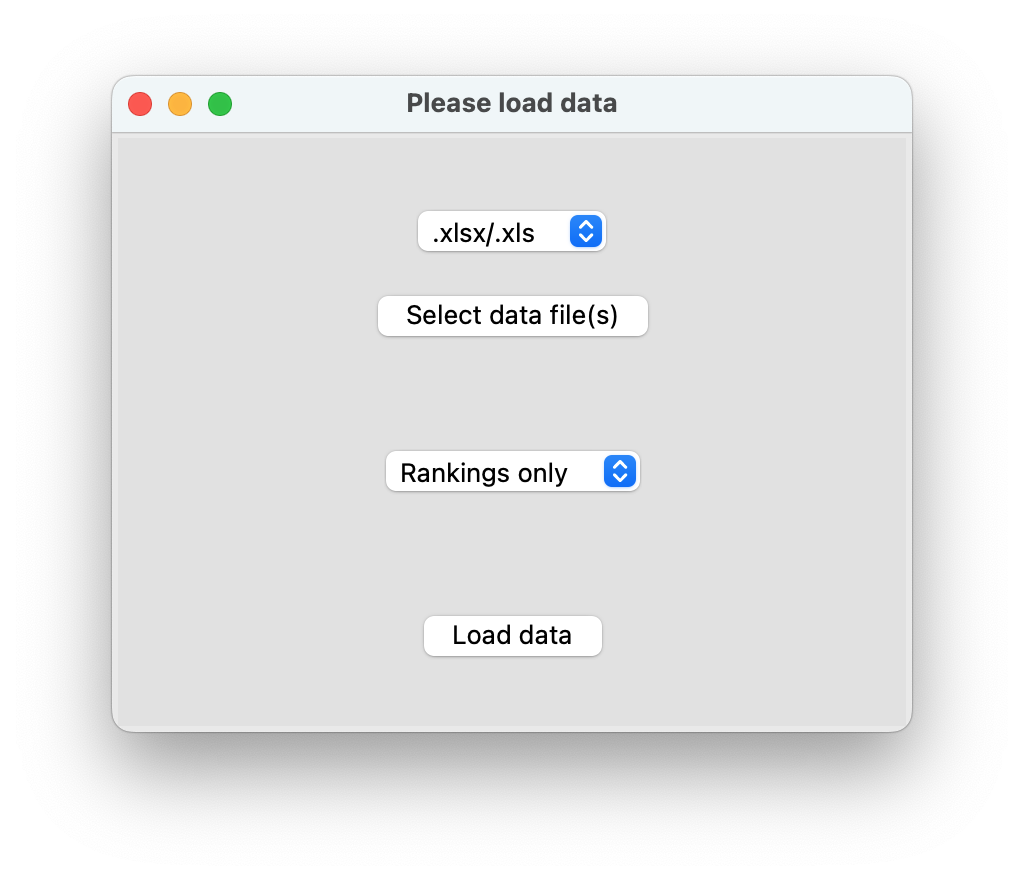
\includegraphics[width=0.5\textwidth]{art/loading.png}
			\caption{Window for loading data.}\label{fig:loading}
		\end{center}
	\end{figure}

The option menu with default type \texttt{.xlsx/.xls} specifies the format of data.
If \texttt{.xlsx/.xls} is selected, the excel file can have multiple sheets depending on the type of the data and the file whould be loaded.
If \texttt{.csv} is selected, the directory containing the .csv files should be selected.

The button ``Select data file(s)'' will open a window for selecting directory/file.
After selecting, 
the line ``Data Selected!'' will appear below the button.

The option menu with default type \texttt{Rankings only} specifies the type of data.
There are three options: ``Rankings only'', ``Ratings only'' and ``Ratings and Rankings''.

Table~\ref{tab:input} concludes the input document needed under each combination:

\begin{table}[H]
  \centering
  \scriptsize
  \begin{tabular}{l|l|p{3.5cm}|l}
    \toprule
    Datatype & File format & Document required & Models\\
    \midrule
    \multirow{2}{*}{\texttt{Rankings only}} & \texttt{.xlsx/.xls} & Sheet names: ``Rankings'', ``Attributes''
    & \multirow{2}{*}{Mallows, GMM,  RIM, Borda} \\
    \cline{2-3}
    & \texttt{.csv} & ``rankings.csv''& \\
    \hline
    \multirow{2}{*}{\texttt{Ratings only}} & \texttt{.xlsx/.xls} & Sheet names: ``Scores'', ``Attributes''
    & \multirow{2}{*}{Borda} \\
    \cline{2-3}
    & \texttt{.csv} & ``ratings.csv'' & \\
    \hline
    \multirow{2}{*}{\texttt{Ratings and Rankings}} & \texttt{.xlsx/.xls} & Sheet names: ``Scores'',``Ratings'', ``Attributes'' & \multirow{2}{*}{Mallows, GMM, RIM, Landmarks, Borda} \\
    \cline{2-3}
    & \texttt{.csv} & ``ratings.csv'', ``rankings.csv''& \\
    \bottomrule
  \end{tabular}
  \caption{Table of input types and document(s) required.}\label{tab:input}
\end{table}

After inputting the document(s), click on ``Load data'' to load in the dataset.

The excel file should be arranged as follows:
\begin{itemize}
  \item Sheet ``Scores'': The first column contains the names of the candidates/proposals; the second column contains the names of the reviewers; the rest of the columns represent different features.
  \item Sheet ``Rankings'': The columns represent rankings of items for all reviewers (using reviewer names). The names of the columns should match the names of the reviewers in ``Rankings'', if ``\texttt{Ratings and Rankings}'' is selected.
  \item Sheet ``Attributes'': Has two columns ``Categories'' and ``Type''. ``Categories'' contain all features in the ``Scores'' sheet and ``Type'' specifies whether it is a sub-rating (``Ratings''), text commment (``Text'') or overall rating (``Main'').
\end{itemize}

Note that here ``overall rating'' means the ratings we use to generate the consensus rankings.

\section{Main canvas}

  \begin{figure}
    \begin{center}
      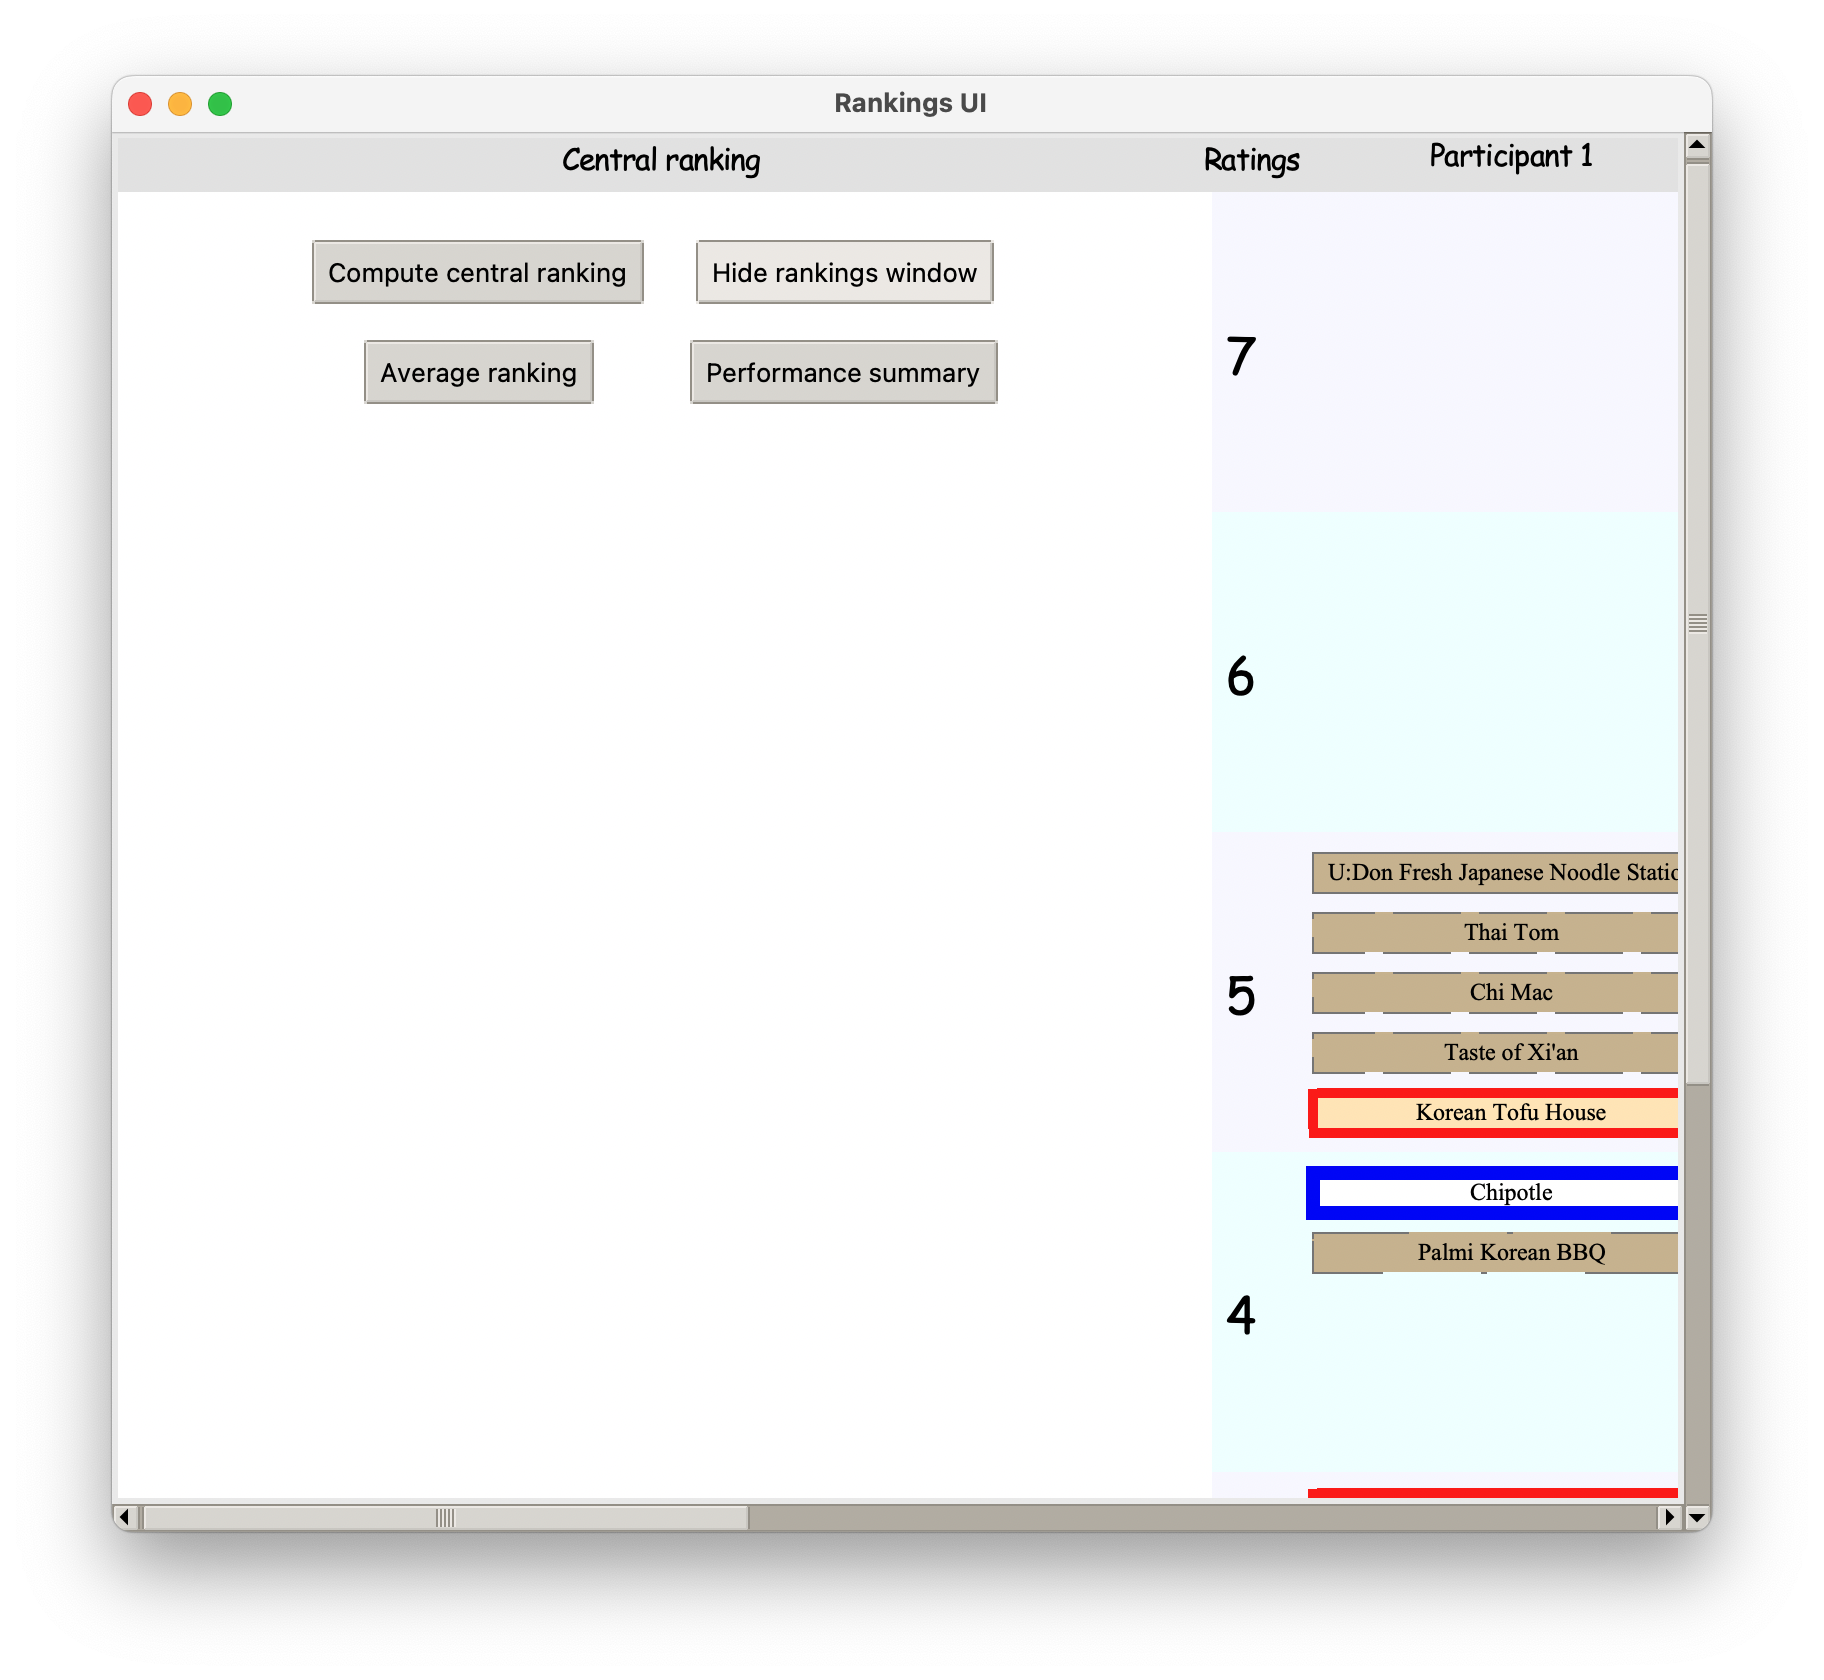
\includegraphics[width=0.7\textwidth]{art/base.png}
      \caption{Main canvas of the GUI.}\label{fig:base}
    \end{center}
  \end{figure}

On the left-hand side, the four buttons have the following functions:

\begin{itemize}
\item Button ``Compute consensus ranking'': open the window for computation under models in Section~\ref{subsec:consensus}.

\item Button ``Hide rankings window'': hide the consensus rankings window temporarily while still saving the results.

\item Button ``Average ranking'': provide basic statistics based on the consensus rankings computed using the current model.

\item Button ``Performance summary'': open the performance summary window in Section~\ref{subsec:modelcompare}. Should be used after computing the results.
\end{itemize}

On the right-hand side, the columns represent all the reviewers and the rows represent the 
overall ratings. The item boxes are displayed according to the ratings.

\begin{itemize}
\item Single clicking an item box will color the same item for all reviewers so that the user can see the variation among reviewers.

\item Right clicking the item boxes will show the option menu in Figure~\ref{fig:items_menu}.
The options are:
  \begin{itemize}
      \item Filter: open a window that can filter certain entries.
      \item Rating Details: open a window that contains all detailed sub-ratings.
      \item Review Text: open a window that contains the reviews in text.
      \item Proposal Details: open a window that contains the proposal details. {\color{red} Not currently used.}
      \item Exit: exit the option menu.
  \end{itemize}

\item Double clicking an item will shift the entire column with the column on its left if exists.
So the order of the reviewers can be changed.
\end{itemize}

  \begin{figure}
    \begin{center}
      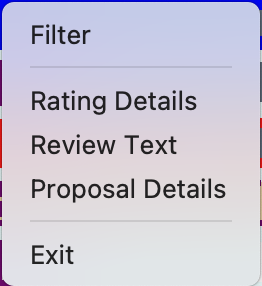
\includegraphics[width=0.2\textwidth]{art/item_menu.png}
      \caption{Option menu after right clicking the item.}\label{fig:items_menu}
    \end{center}
  \end{figure}

  \begin{figure}
    \begin{center}
      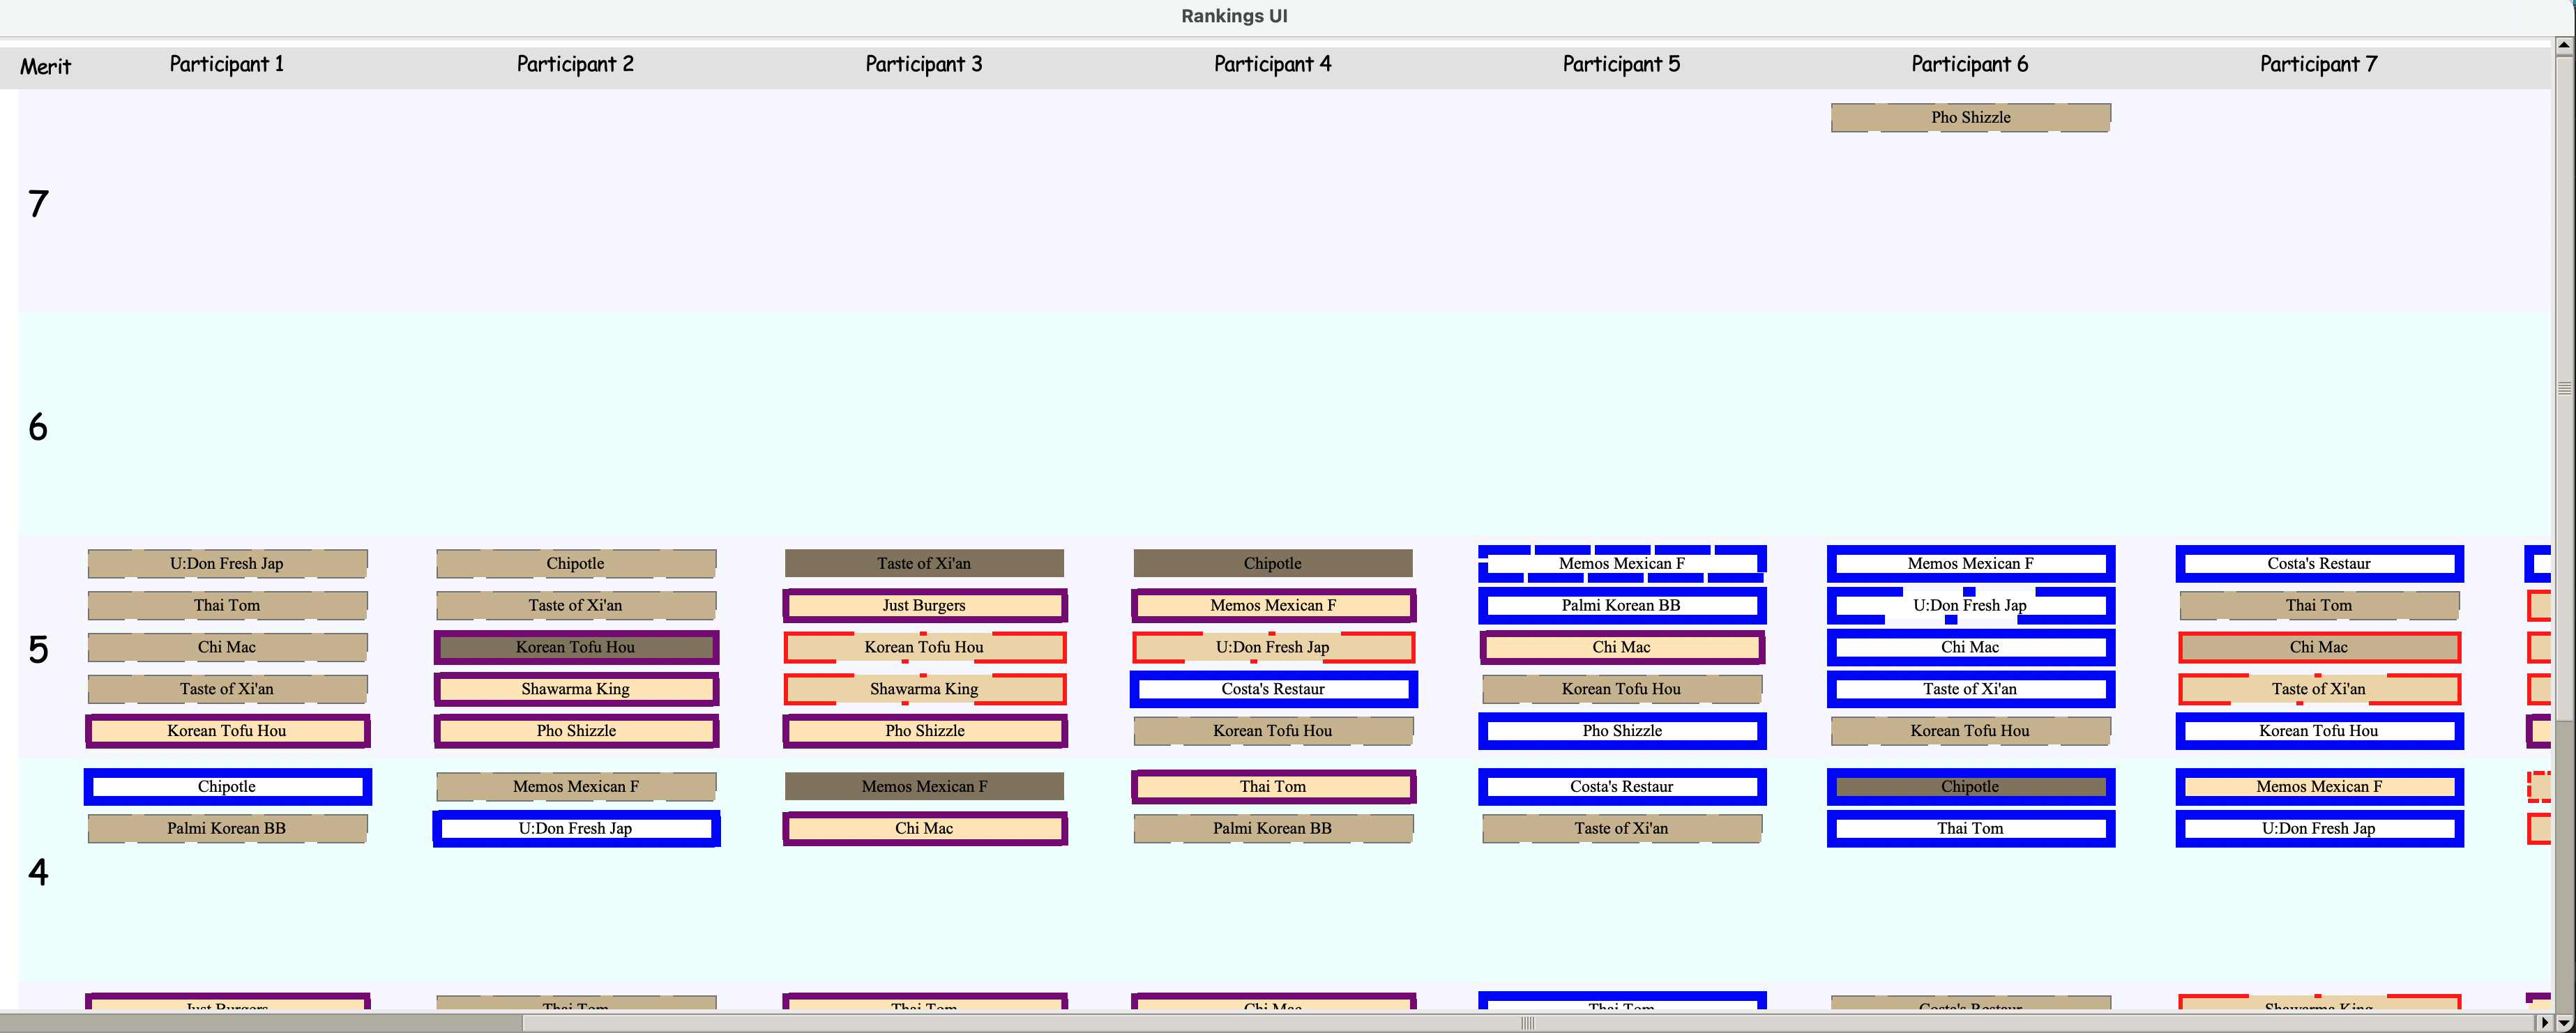
\includegraphics[width=0.95\textwidth]{art/items.png}
      \caption{Item boxes on the canvas.}\label{fig:items}
    \end{center}
  \end{figure}


\section{Legends}
The legend window displays a table of the graphical attributes and the corresponding features they represent,
see Figure~\ref{fig:legend}.

Double clicking any row in this table will open a window that shows the details of that feature,
see Figure~\ref{fig:legend_sub}.

On top of the window, there is a button called ``Change Graphical Attributes'' for changing their assignments.
The new window is in Figure~\ref{fig:legend_change}.


  \begin{figure}[h]
    \begin{center}
      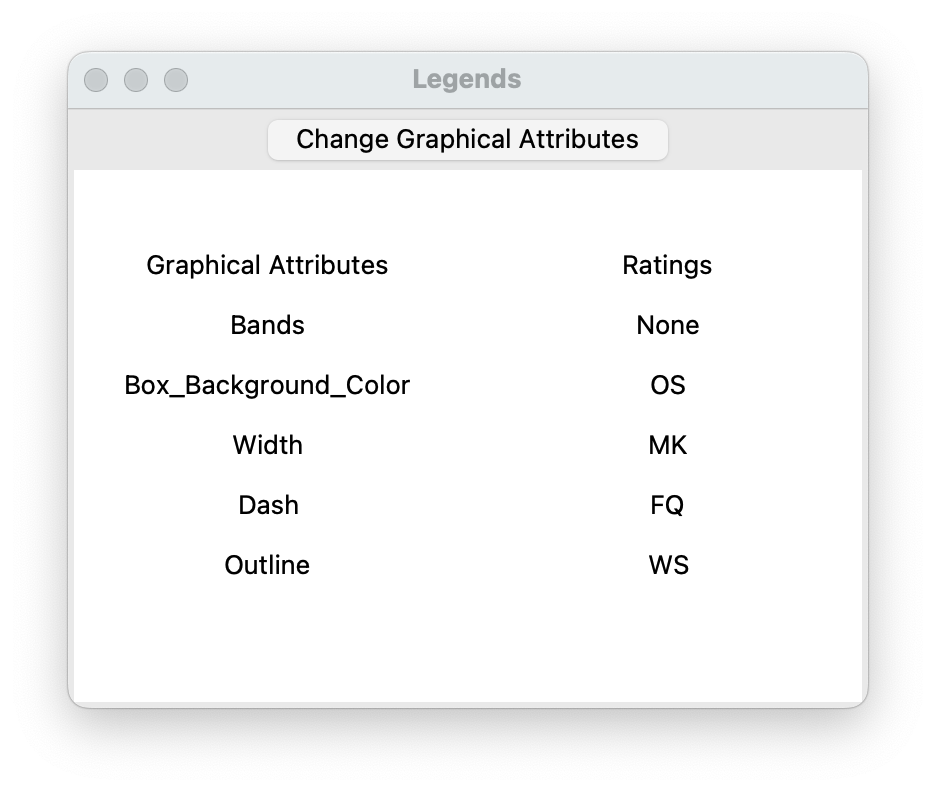
\includegraphics[width=0.35\textwidth]{art/legend.png}
      \caption{The legend window.}\label{fig:legend}
    \end{center}
  \end{figure}


  \begin{figure}[h]
    \begin{center}
      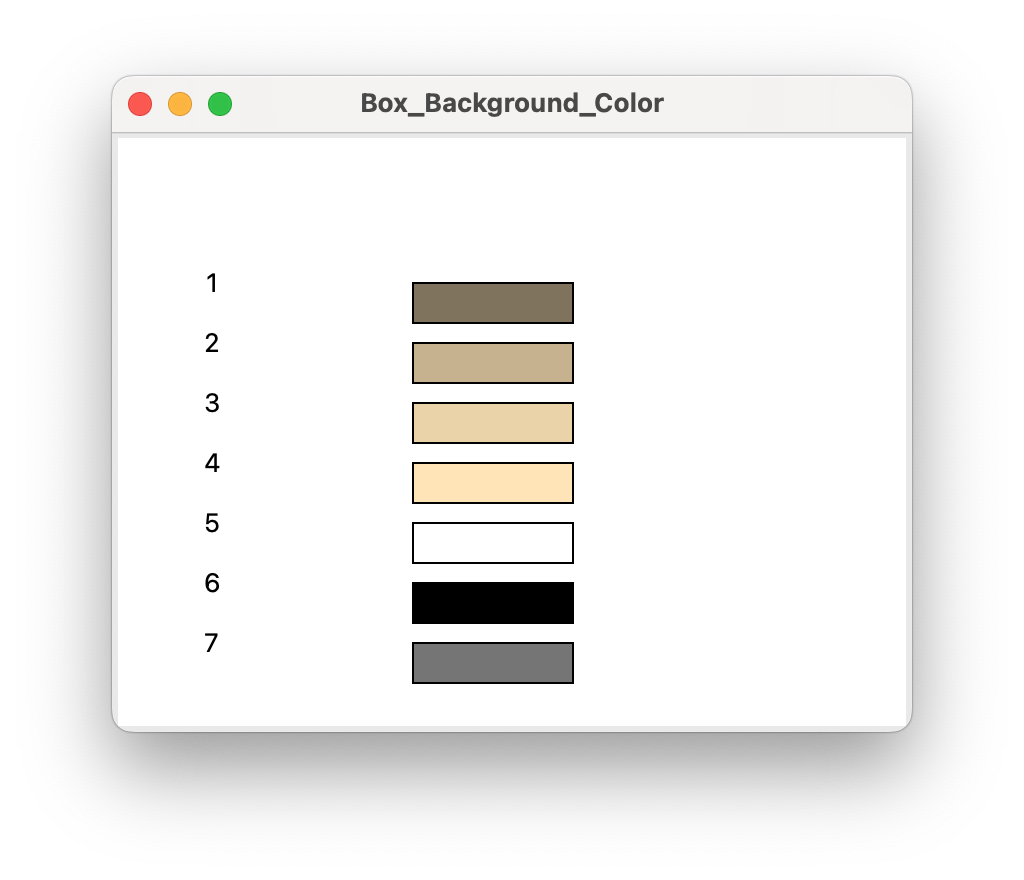
\includegraphics[width=0.35\textwidth]{art/legend_sub.png}
      \caption{A sub window for the box color in the legend.}\label{fig:legend_sub}
    \end{center}
  \end{figure}

  \begin{figure}[h]
    \begin{center}
      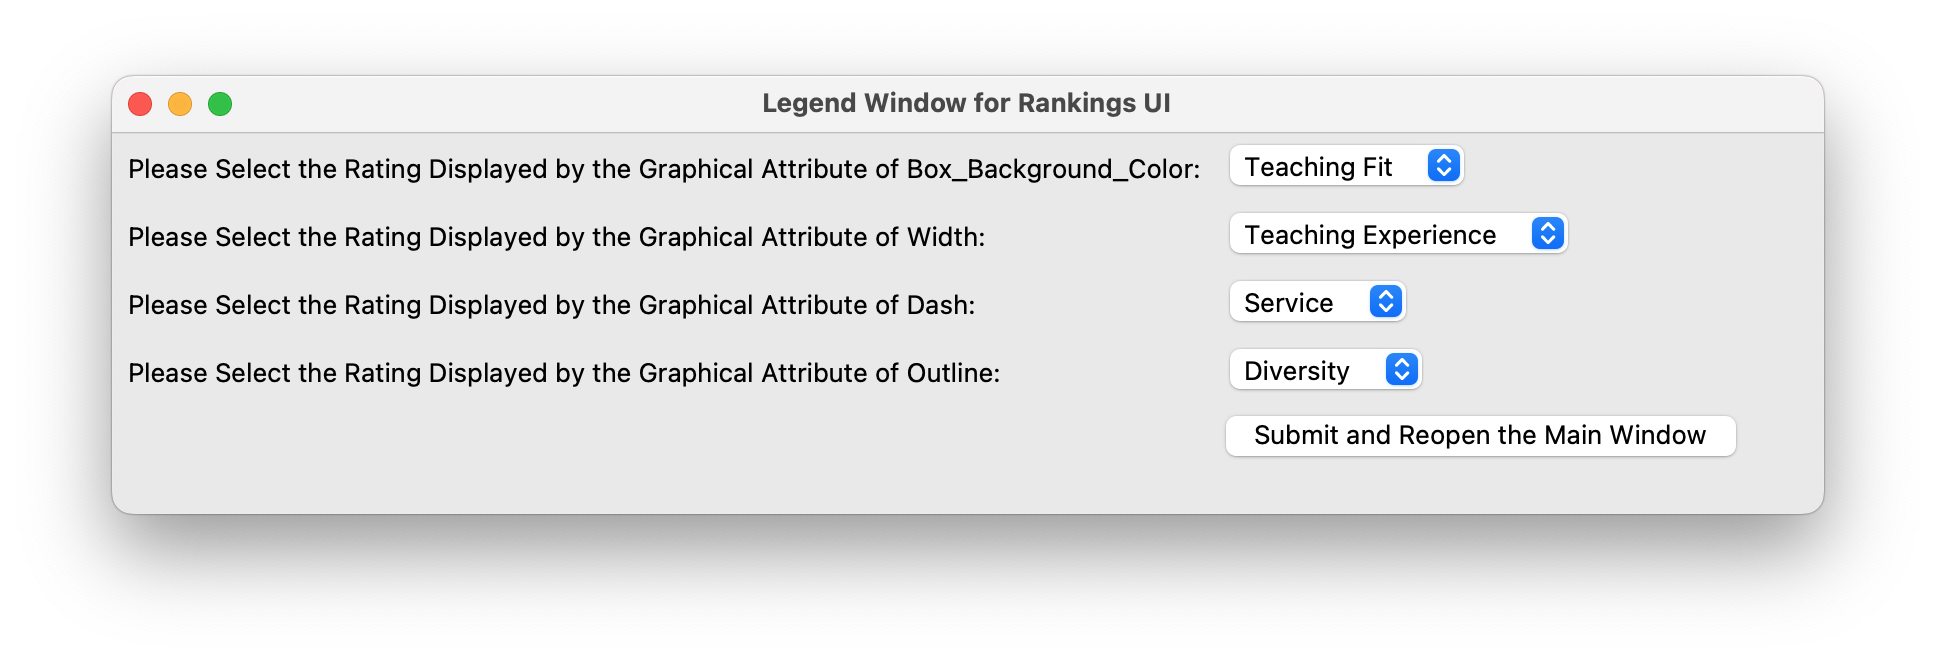
\includegraphics[width=0.8\textwidth]{art/legend_change.png}
      \caption{Window for changing graphical attributes.}\label{fig:legend_change}
    \end{center}
  \end{figure}

\chapter{Concensus rankings}
\section{Consensus rankings window}\label{subsec:consensus}

The window has an area for computing the rankings under different models.
\begin{itemize}
  \item It starts with an option menu with the model options under the current data type.
  \item Button ``Set working directory'': choose a directory for saving model outputs. The selected path will be printed next to the button.
  \item Button ``Load Model Results'': choose a \texttt{.json} file with saved model results. After loading, the saved results would re-display on the window.
  \item Button ``Compute Consensus Ranking'': compute consensus rankings for the chosen model.
  \item Button ``Reset parameter(s)'': if there are parameter(s) for the model, the default values will be reset.
  \item Button ``Save models'': save the computed model results in a \texttt{.json} file.
\end{itemize}
  \begin{figure}
    \begin{center}
      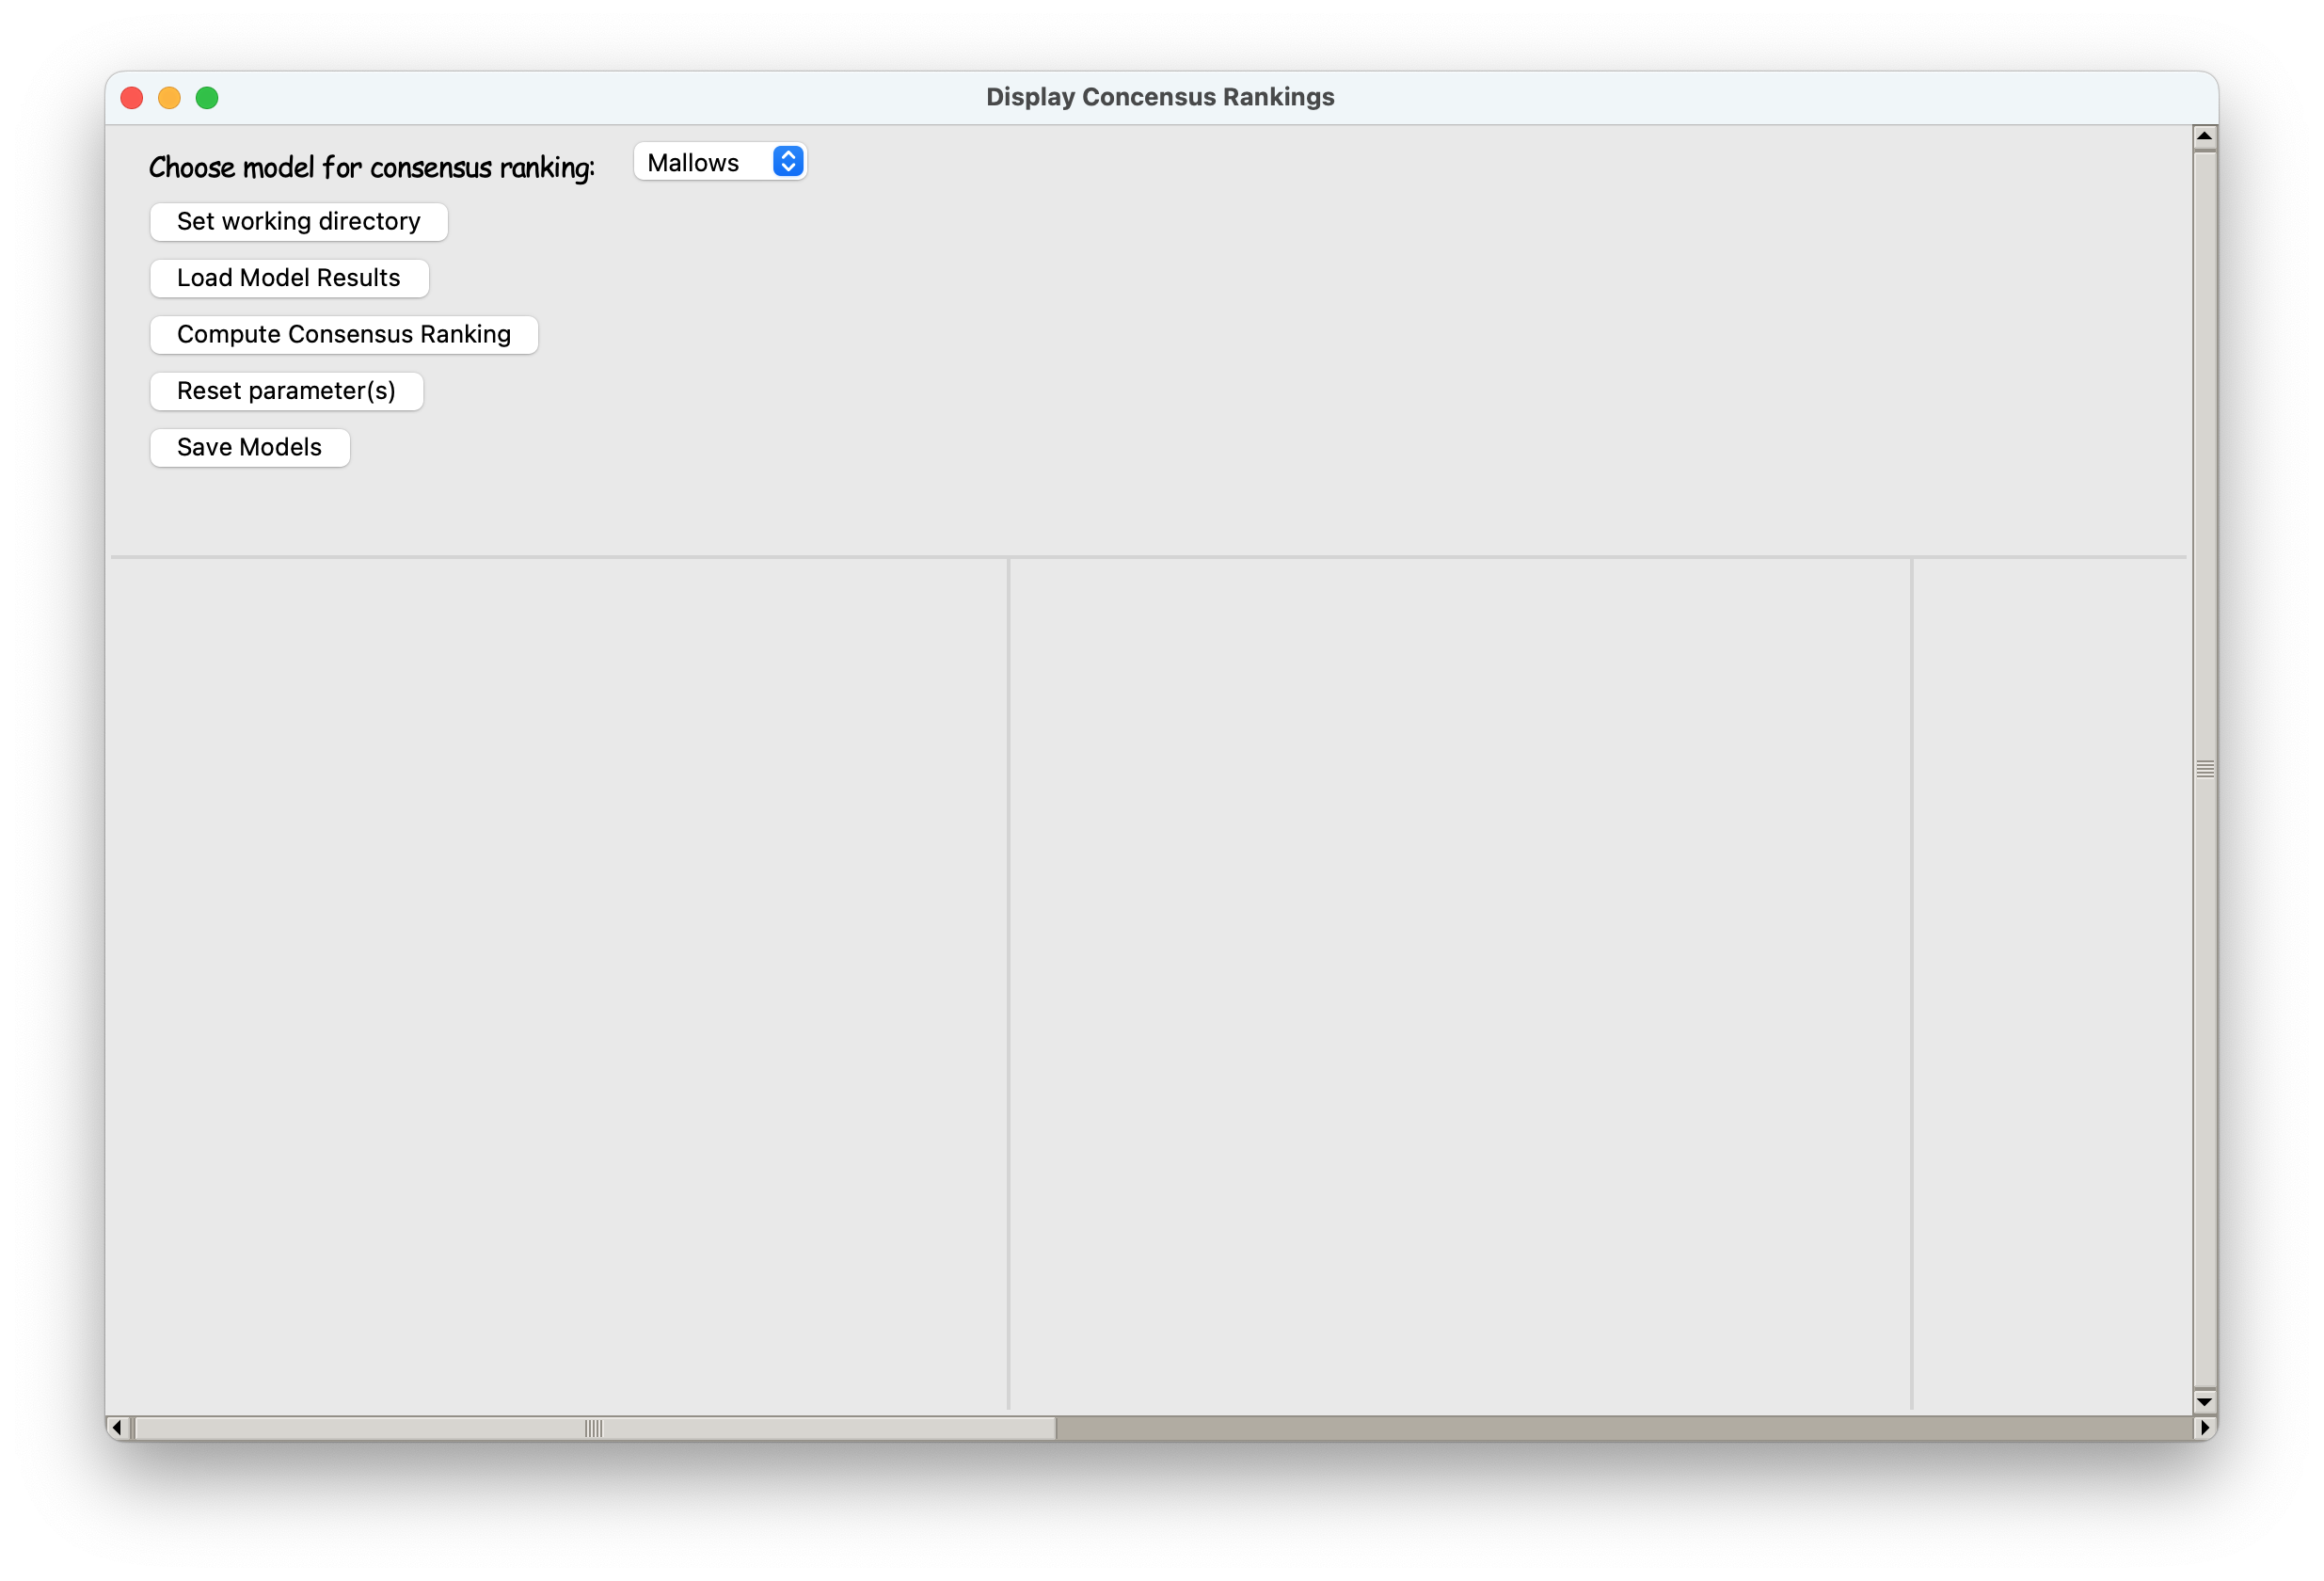
\includegraphics[width=0.9\textwidth]{art/consensus.png}
      \caption{Window for consensus rankings.}\label{fig:consensus}
    \end{center}
  \end{figure}

\section{Model details}

The user may select among the following models for computation.
The default choice is the Mallows model, 
which is very fast and has a single paramter $\theta$.
Revisit Table~\ref{tab:input} for the models available under different data types.

\begin{table}[H]
  \centering
  \scriptsize
  \begin{tabular}{l|p{2cm}|p{6cm}|l}
    \toprule
    \textbf{Model} & \textbf{Parameter(s)} & \textbf{Results displayed} & \textbf{Reference(s)} \\
    \midrule
    Mallows &  & cost; consensus rankings; $\exp(-\theta)$ & \cite{mallows1957}\\[0.5em]
    \hline
    RIM & iterations: no. of iterations temp: tuning parameter for convergence & cost; tree plot; $\exp(-\theta)$ & \cite{meek2014rim}\\[0.5em]
    \hline
    GMM & & cost; consensus rankings; $\exp(-\theta_i)$ & \cite{fligner1986distance}\\[0.5em]
    \hline
    Landmarks & & cost; consensus rankings; $\exp(-\theta_i)$ & \\[0.5em]
    \hline
    Borda & & consensus rankings; column sums of Q matrix (rankings and/or ratings) &\\
    \bottomrule
  \end{tabular}
  \caption{Table of parameters, results displayed and references for the concensus ranking models used.}\label{tab:model}
\end{table}


The models used are summarized in Table~\ref{tab:model}.

For Borda, if both rankings and ratings are provided, the rankings based on rankings (increasing) and ratings (decreasing) will be computed.
They should agree with each other.

For users not familiar with the details of the model, we also highlight important properties of the models:


\begin{table}[H]
  \centering
  \scriptsize
  \begin{tabular}{l|p{3cm}|p{3cm}|p{3cm}}
    \toprule
    \textbf{Model} & \textbf{Computation Speed} & \textbf{Cost} & \textbf{Interpretability} \\
    \midrule
    Mallows & Very fast & Higher because of its simplicity &  \\[0.5em]
    \hline
    GMM & Fast & Lower than Mallows & \\[0.5em]
    \hline
    RIM & Moderate, depending on number of iterations & Lower, complex model & Tree plot available\\[0.5em]
    \hline
    Landmarks & Moderate, depending on number of iterations &  & Can utilize both rankings and ratings information \\[0.5em]
    \hline
    Borda & Very fast & --- & Intuitive \\
    \bottomrule
  \end{tabular}
  \caption{Table of comparisons between different models.}\label{tab:model}
\end{table}

Faster models might be preferred if the number of items or the number of bootstrap samples is large.



\section{Model summary window}\label{subsec:modelcompare}
Upon opening the model comparison window, 
on the left-hand side we can first select the window(s) 
we wish to compare.
Only models computed in the model comparison window will be included.
See Figure~\ref{fig:summary1}.


\begin{figure}
  \begin{center}
    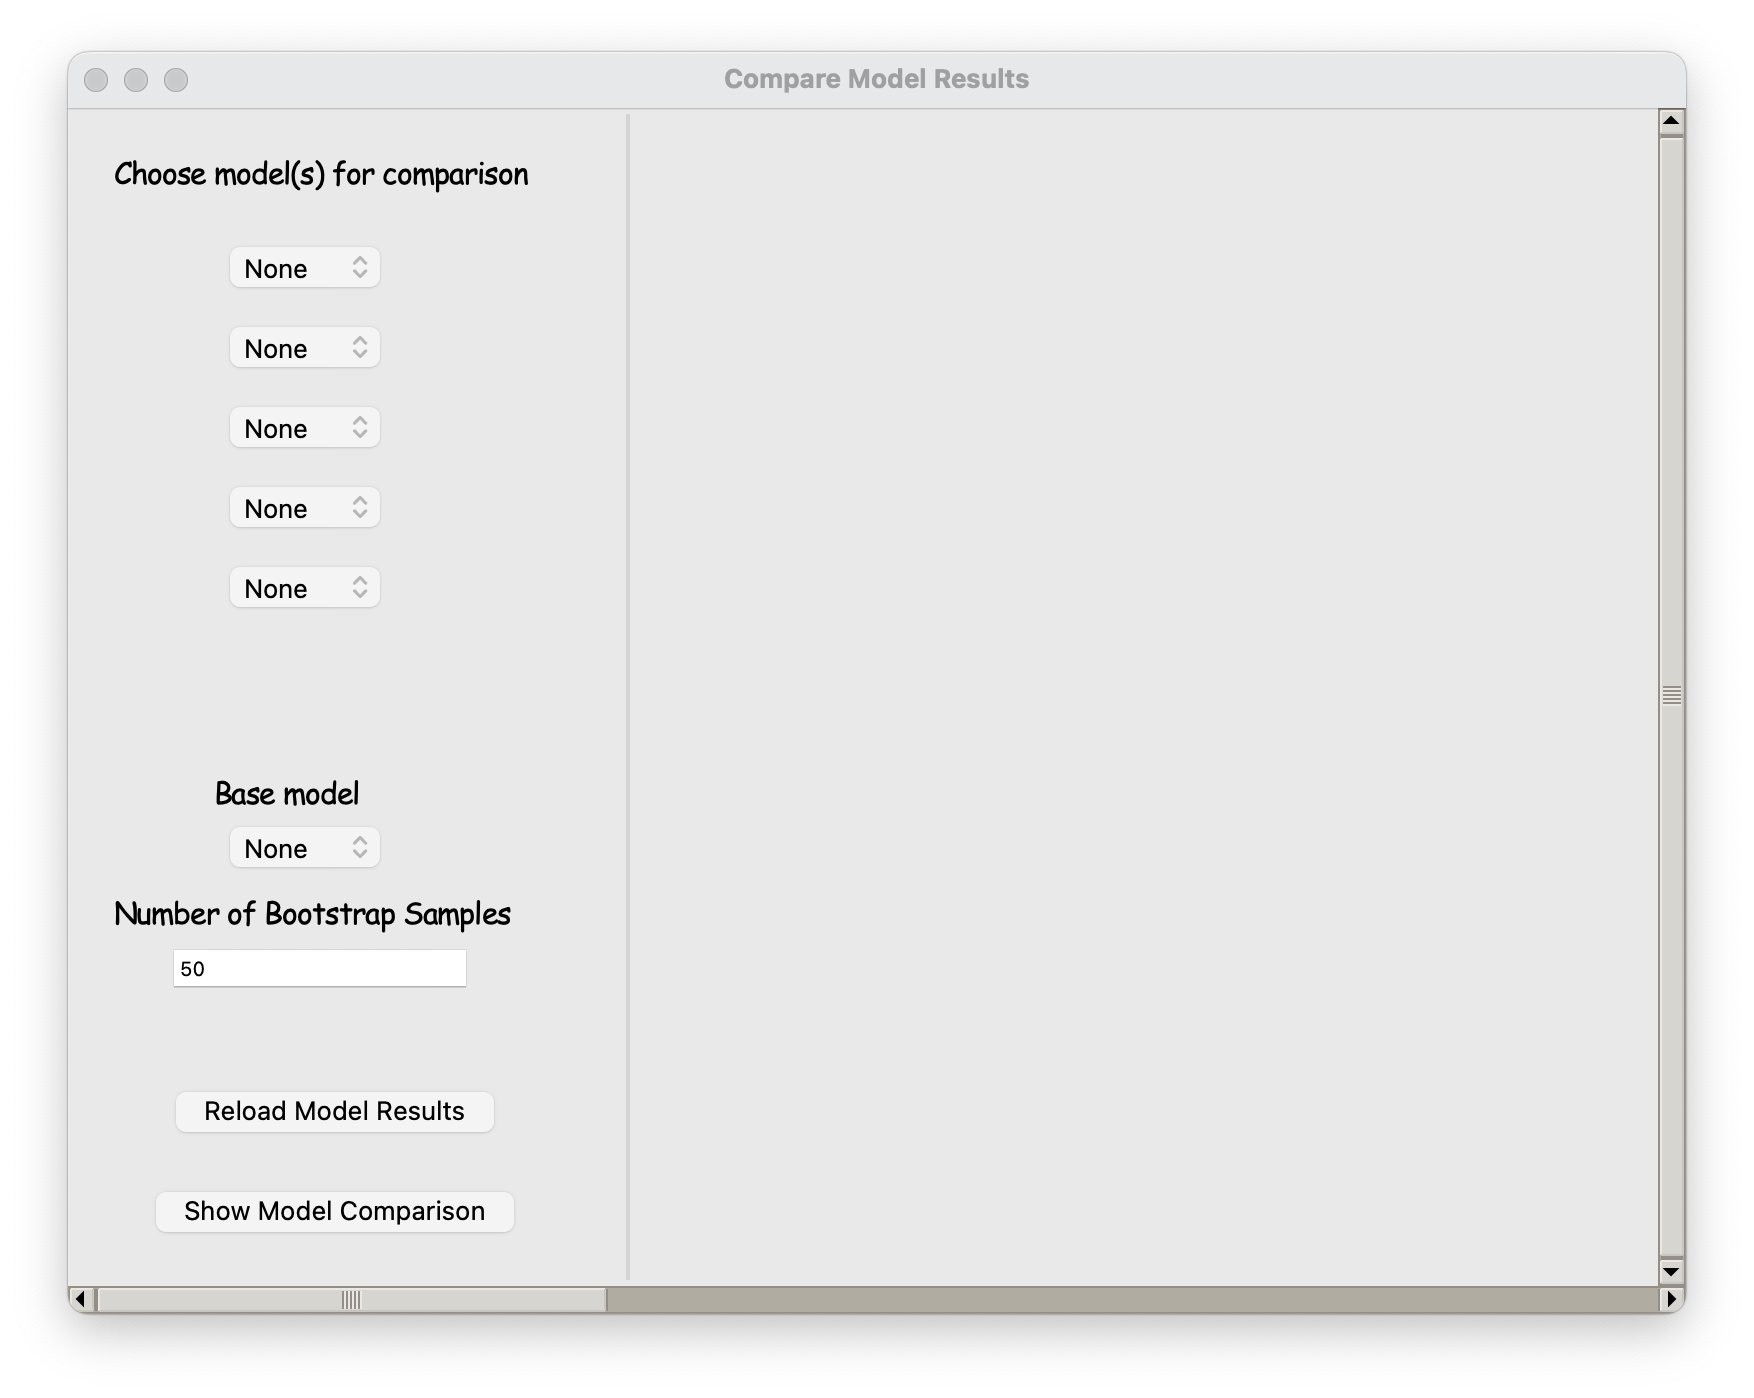
\includegraphics[width=0.8\textwidth]{art/summary_1.png}
    \caption{Selecting model(s) for comparison.}\label{fig:summary1}
  \end{center}
\end{figure}


We then need to select a ``base'' model used as a benchmark for comparisons across rankings from different models.

The number of bootstrap samples (integer) should be entered for comparing the variation of results among bootstrap samples.

The button ``Reload Model Results'' is used when results from new models are computed and they need to be updated into the summary window.

The button ``Show Model Comparison'' computes the summary of the models which will appear on the right-hand side of the window.


The following results will be displayed, from the first row to the third:
\begin{itemize}
  \item Q matrices computed using the dataset with columns ranked by consensus ranking computed from each model. We expect the color pallette to be smooth for the rankings to be sensible.

  \item Q matrices computed using the set of consensus rankings computed from the bootstrap samples. Items are ranked by the consensus ranking computed from each model. Lighter colors indicate smaller differences between results from bootstrap samples.

  \item Comparison matrix across different models. Lighter color indicates smaller difference between results from different models.
\end{itemize}

The formula for the Q matrix is as follows: 
Let $\mathcal{E} = \{e_1,\ldots, e_n\}$ be the set of items. 
We use $e \prec_\pi e'$ to denote the case that $e$ percedes $e'$ in the permutation $\pi$.
For a dataset containing $N$ sets of rankings $\{\pi_1,\ldots, \pi_N\}$ on $n$ items, 
the $n\times n$ matrix is computed as 
  \begin{equation}
    Q_{e,e'} = \sum_{i=1}^N\mathds{1}_{e \prec_{\pi_i} e'} / N.
  \end{equation}
It is the empirical estimate of the probability of item $e$ perceding $e'$.

The values of the matrices can be checked by placing the mouse on the blocks. 
See Figure~\ref{fig:Qmatrix}.

  \begin{figure}[h]
    \begin{center}
      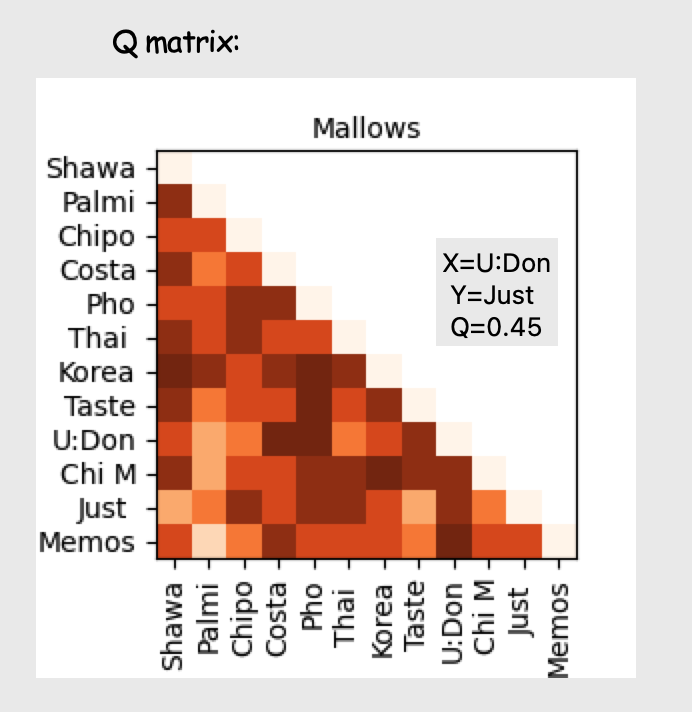
\includegraphics[width=0.5\textwidth]{art/q_matrix.png}
      \caption{Moving the mouse on matrices can check the exact values.}\label{fig:Qmatrix}
    \end{center}
  \end{figure}


\chapter{A simple example}

In this section we present using our GUI to analyse a dataset containing reviews from 12 participants on restaurants in University District of Seattle.
The dataset has both rankings and ratings and is in the format of an Excel file, see 
Figure~\ref{fig:example0}.

  \begin{figure}[h]
    \begin{center}
      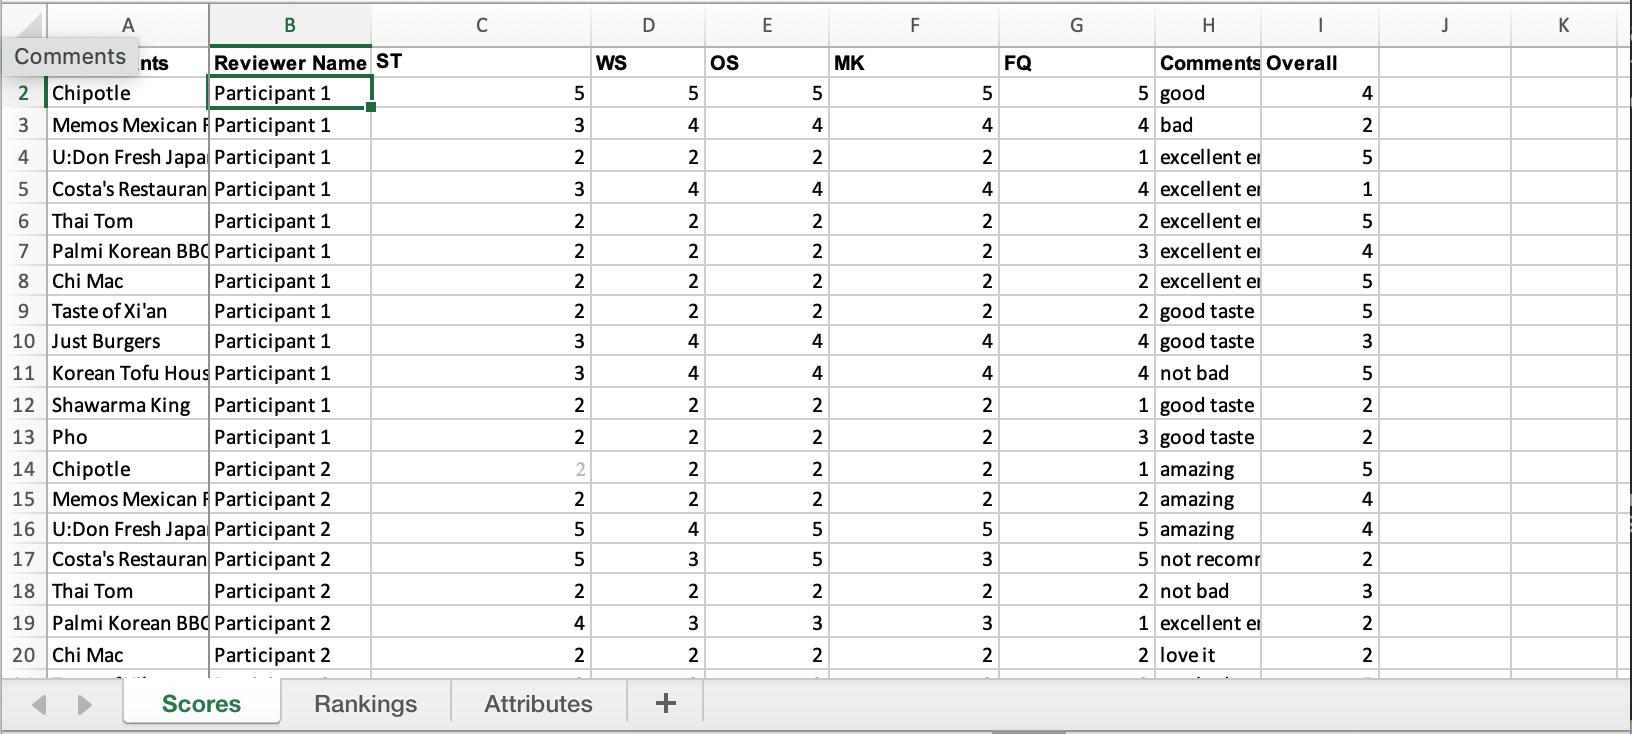
\includegraphics[width=0.95\textwidth]{art/example_data.png}
      \caption{Dataset used in the example.}\label{fig:example0}
    \end{center}
  \end{figure}

The column ``overall'' contains the scores for ranking. There are five sub-ratings denoted as ST, WS, OS, MK and FQ. A text review is in the column ``Comments''.
Then we prepare the configuration file \texttt{config.toml}.
Running the $\texttt{main.py}$ file, 
we load in the data from the following window:

  \begin{figure}[h]
    \begin{center}
      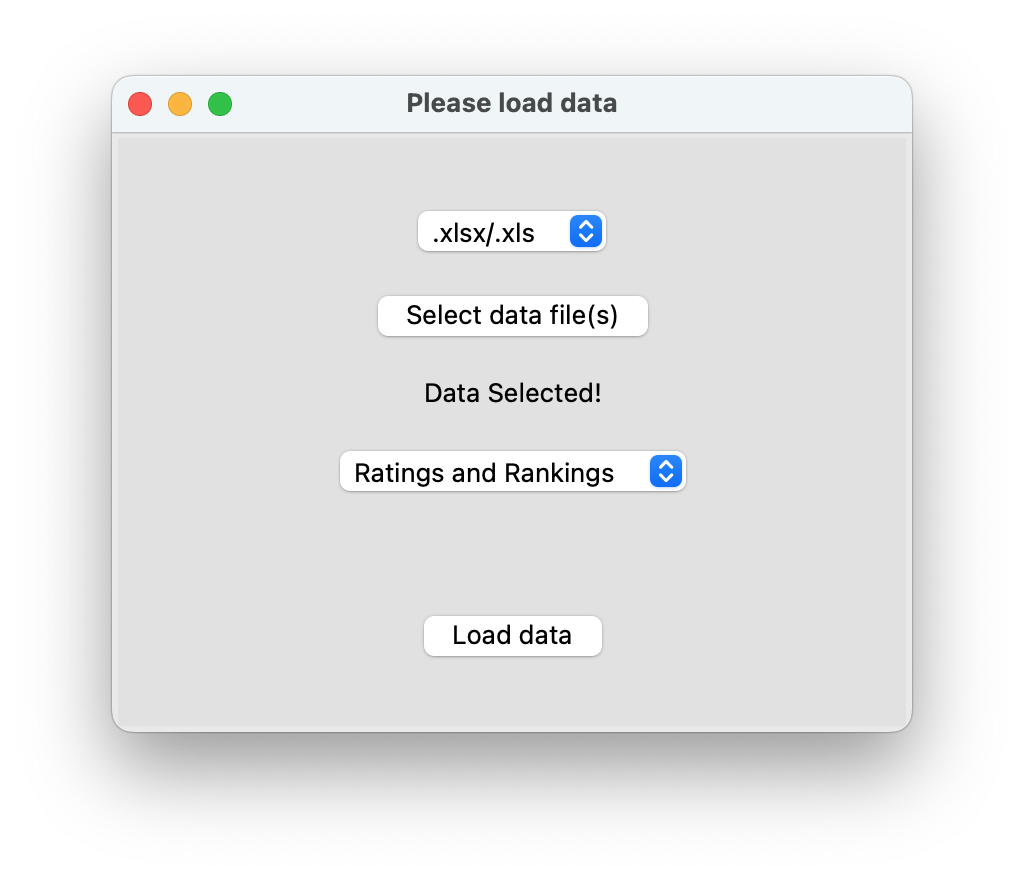
\includegraphics[width=0.5\textwidth]{art/example_1.png}
      \caption{Loading data into the GUI.}\label{fig:example1}
    \end{center}
  \end{figure}

Since we have both rankings and ratings from the data, we select the option \texttt{``Ratings and Rankings''}. 
After pressing ``Load data'', 
the main canvas would pop up as in Figure~\ref{fig:example2}.

  \begin{figure}[h]
    \begin{center}
      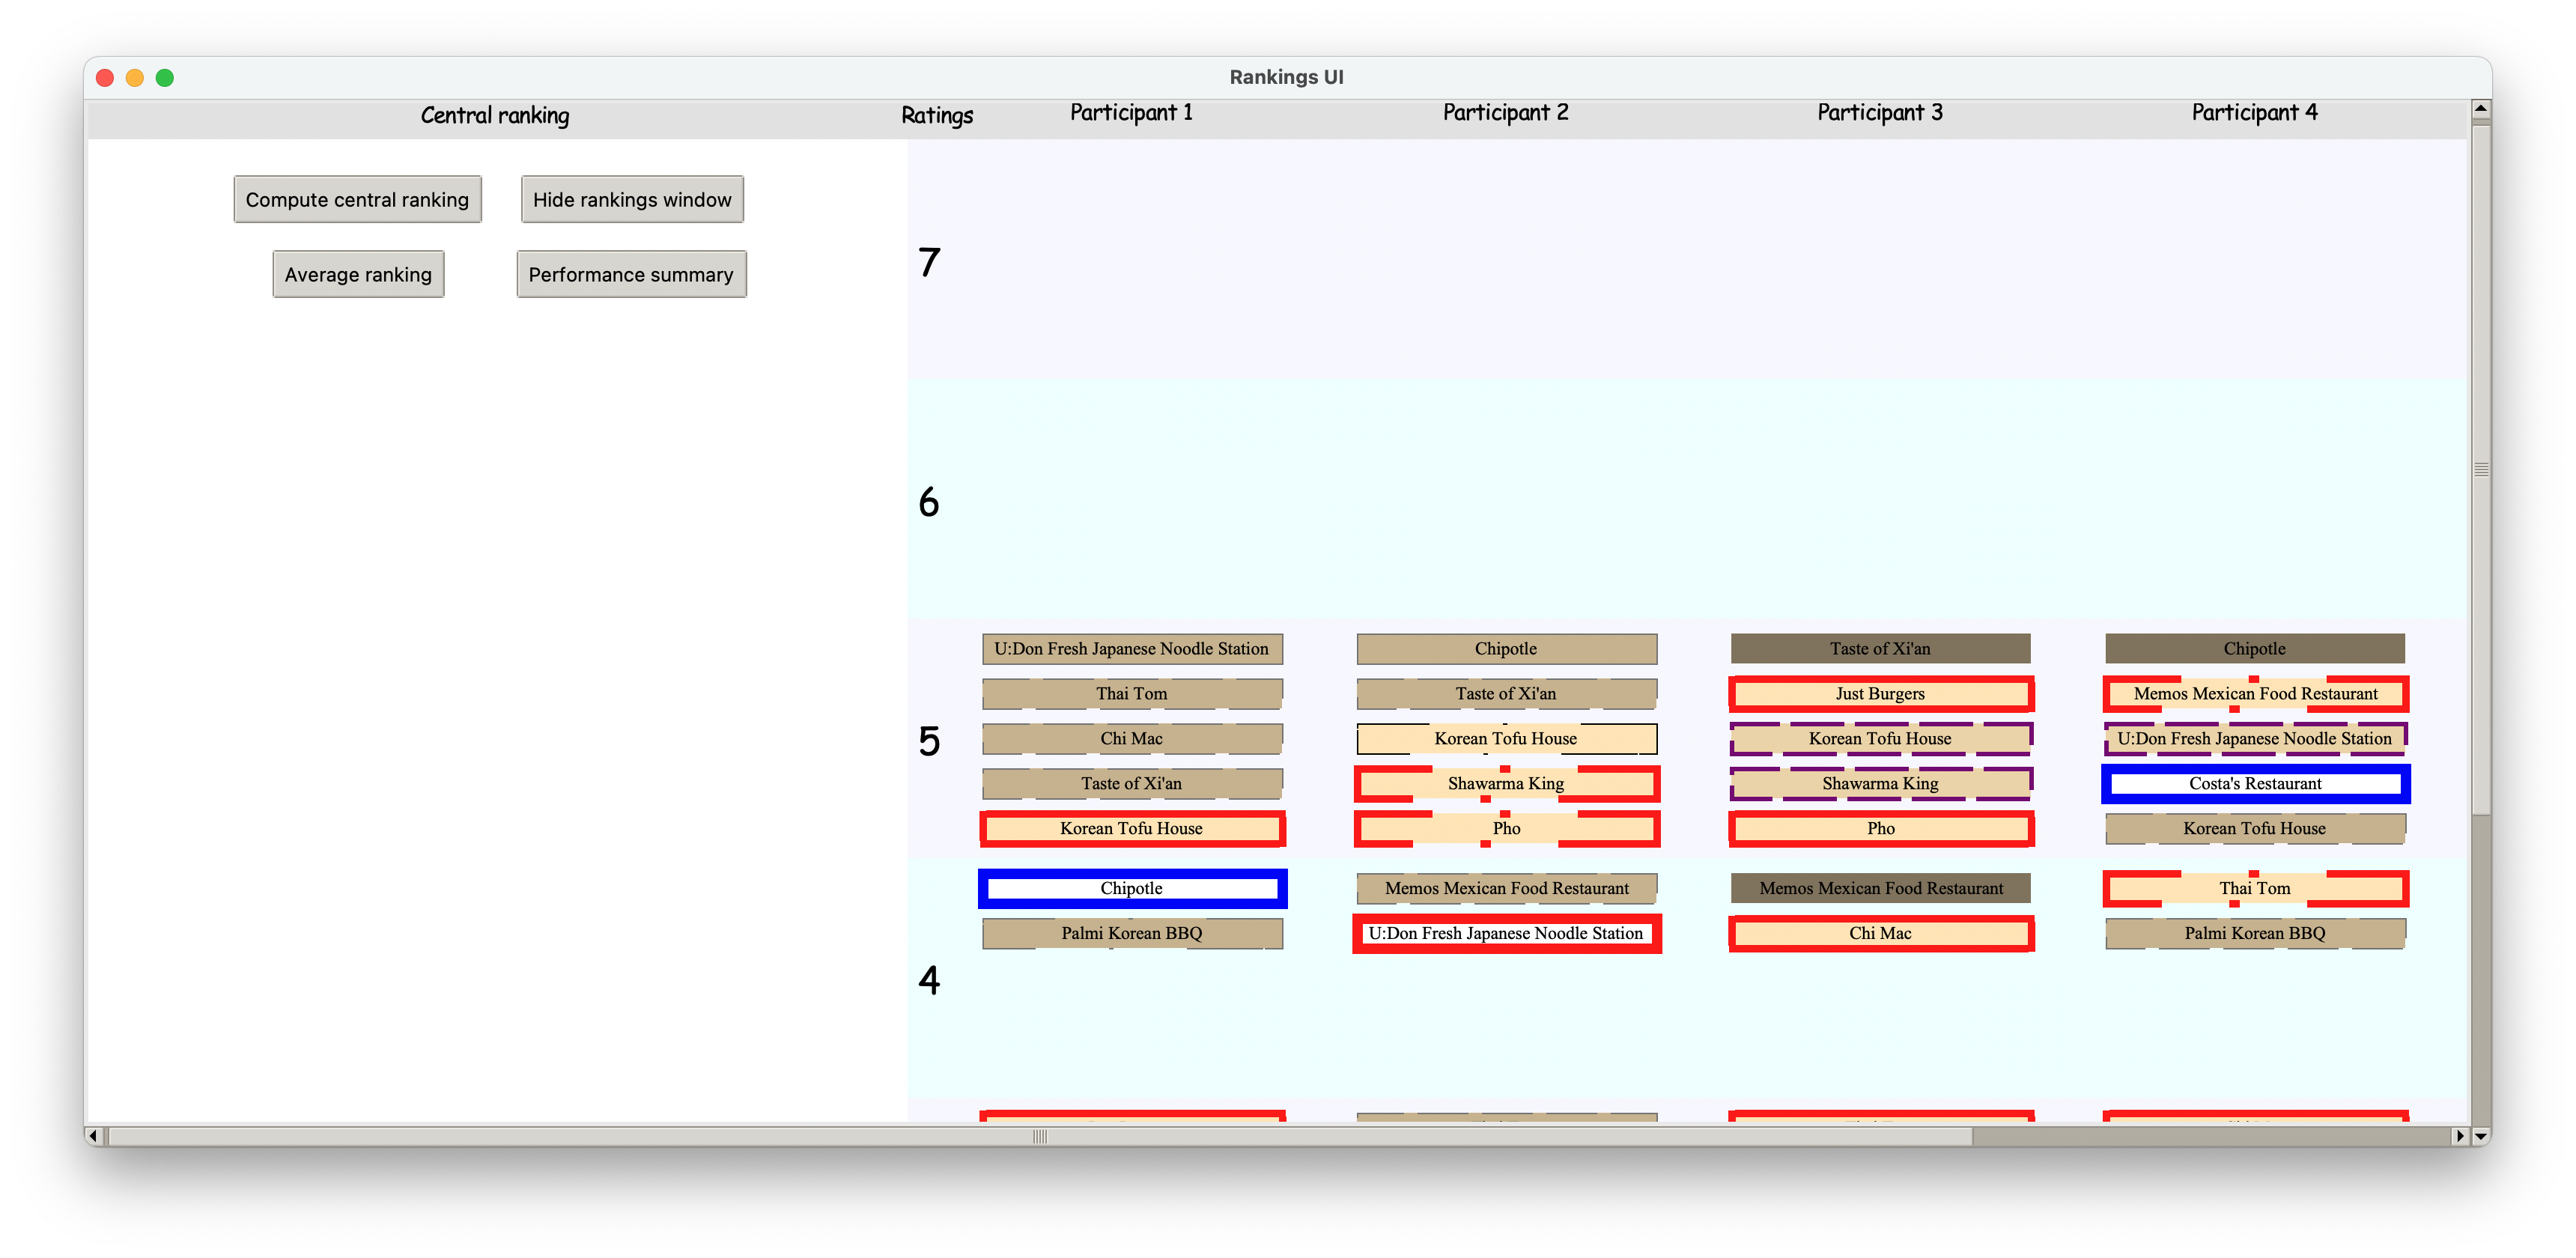
\includegraphics[width=0.95\textwidth]{art/example_2.png}
      \caption{Main canvas for the example.}\label{fig:example2}
    \end{center}
  \end{figure}


Then we can check the details of our items:
if we press an item, for example, Korean Tofu House,
the same candidate will darken in all columns,
see Figure~\ref{fig:darken}. 
If we right-click we can use the option menu to:
\begin{itemize}
  \item Filter the items. By selecting items with minimum scores 2 and maximum 5 for all sub-ratings, the items filtered can be found as in Figure~\ref{fig:filtered}.
  \item Check the sub-ratings. The ``Rating details'' option allows us to check the 4 sub-ratings of an item; see Figure~\ref{fig:sub-ratings.png}.
  \item Check the review texts with the ``Review Texts'' option; see Figure~\ref{fig:review_details.png}.
  \item This example does not include any proposal details; so we skip this function.
\end{itemize}


\begin{figure}[h]
    \centering
    \begin{subfigure}[t]{0.5\textwidth}
        \centering
        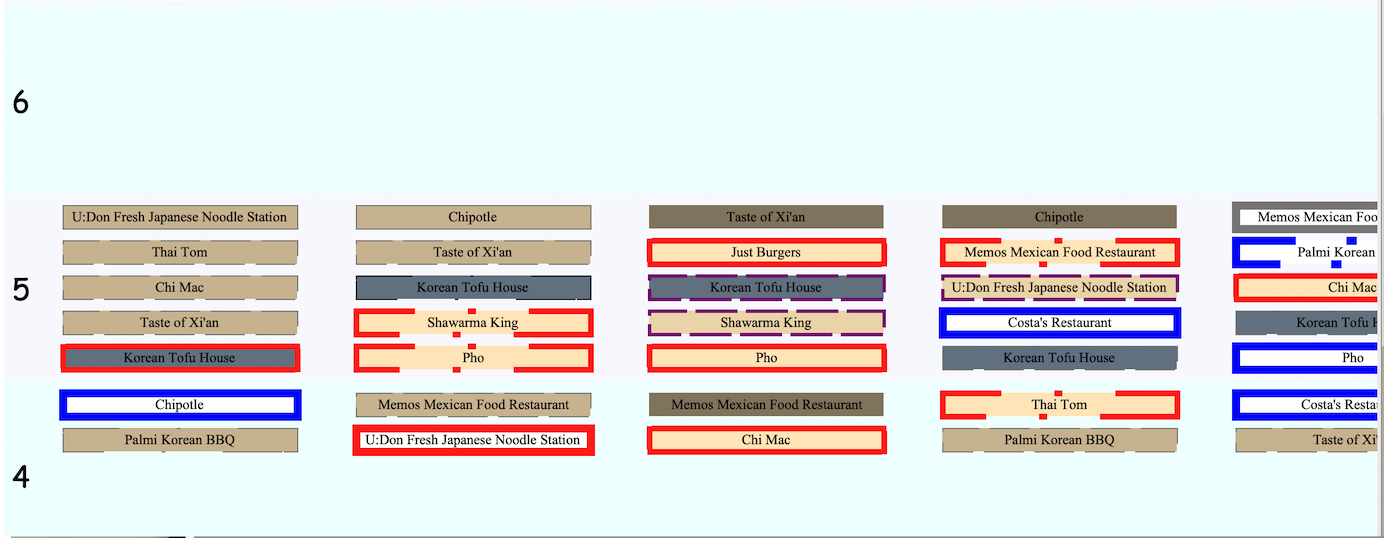
\includegraphics[height=2in]{art/darken.png}
        \caption{\label{fig:darken}}
    \end{subfigure}%
    ~ 
    \begin{subfigure}[t]{0.5\textwidth}
        \centering
        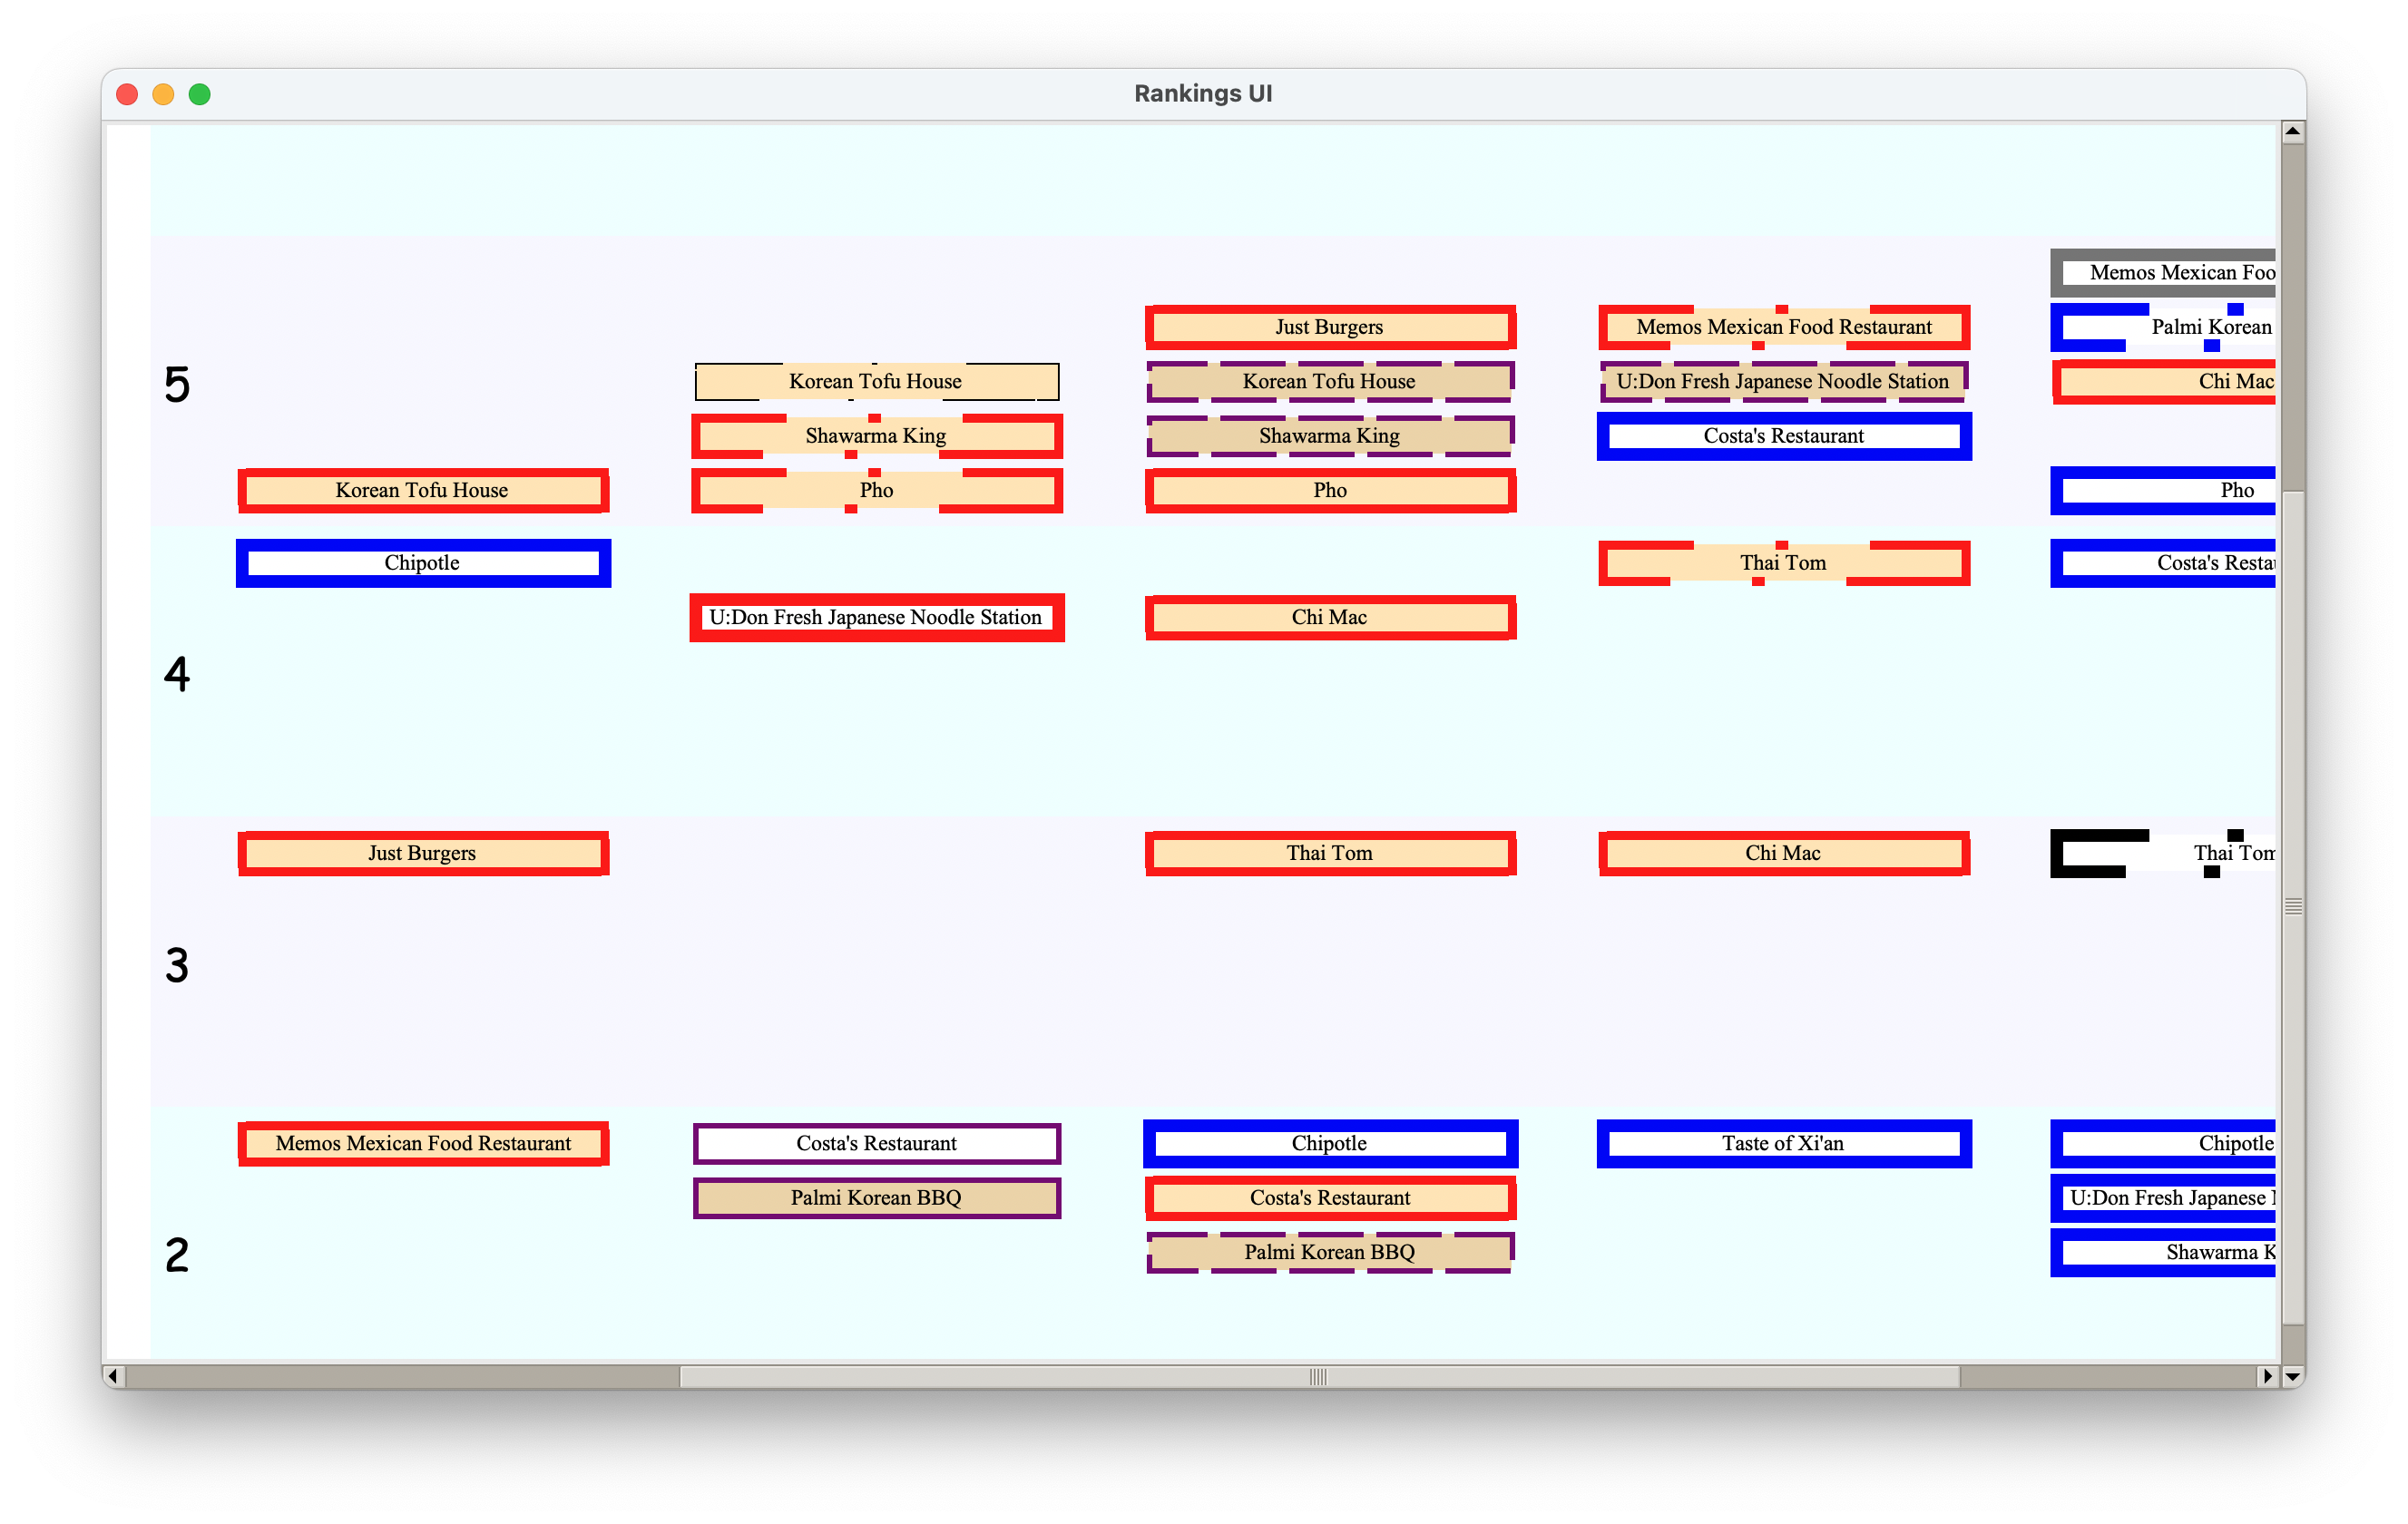
\includegraphics[height=2in]{art/filtered.png}
        \caption{\label{fig:filtered}}
    \end{subfigure}
    ~
    \begin{subfigure}[t]{0.5\textwidth}
        \centering
        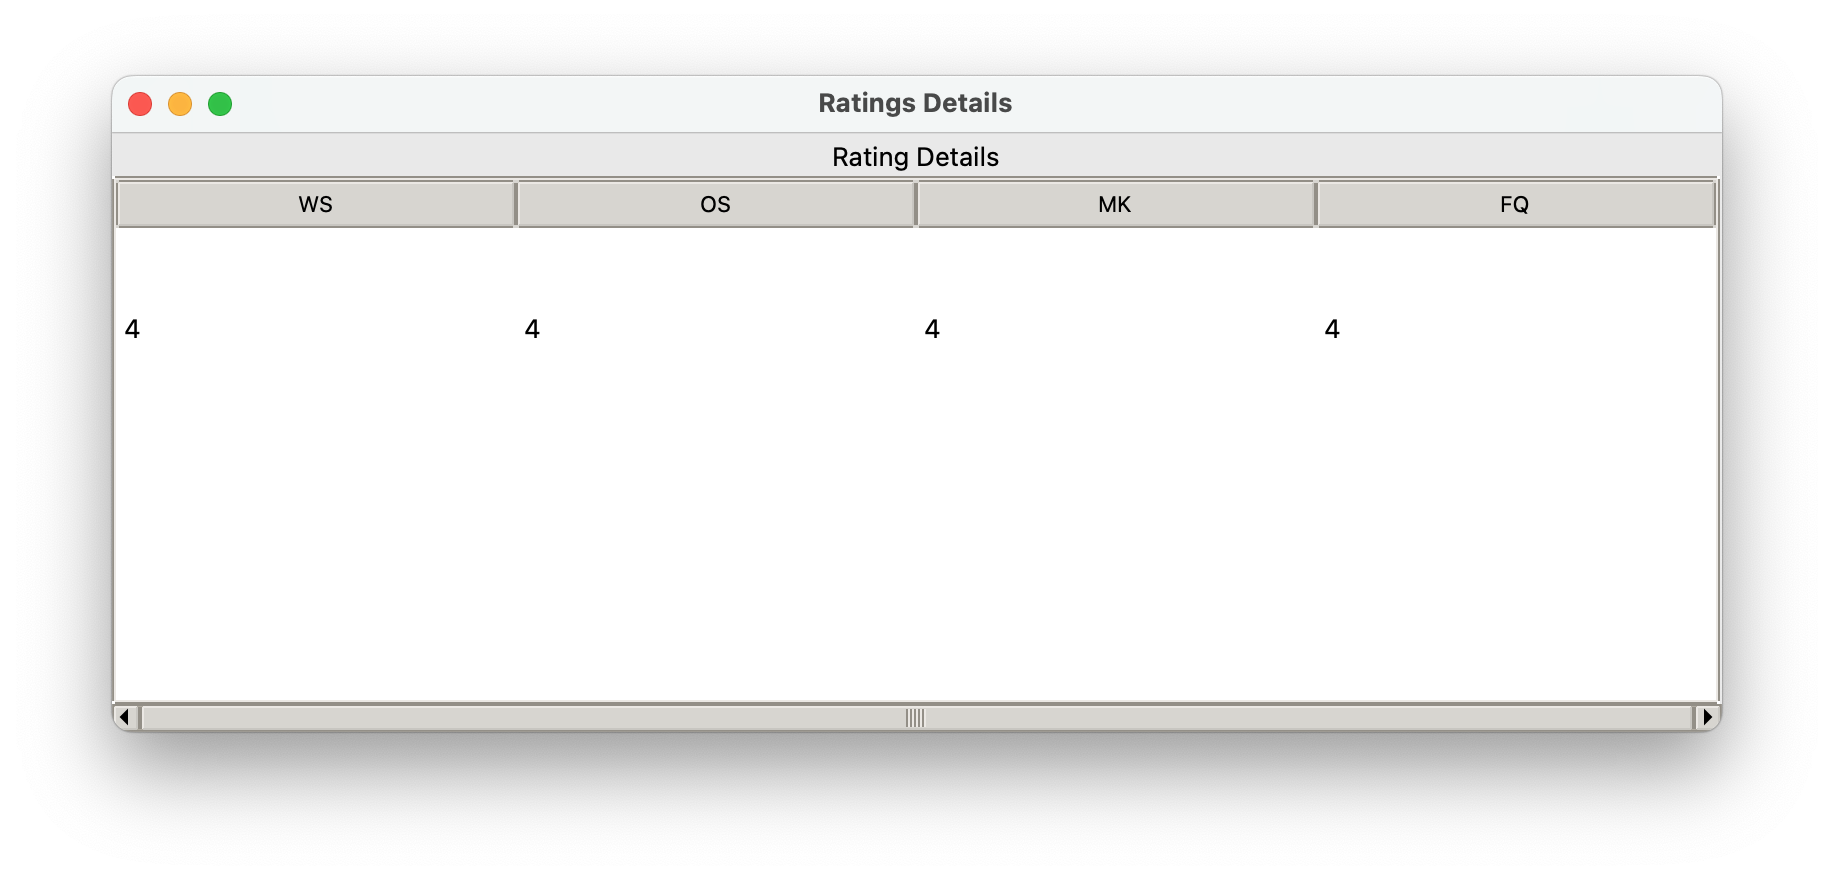
\includegraphics[height=2in]{art/sub-ratings.png}
        \caption{\label{fig:sub-ratings.png}}
    \end{subfigure}%
    ~ 
    \begin{subfigure}[t]{0.5\textwidth}
        \centering
        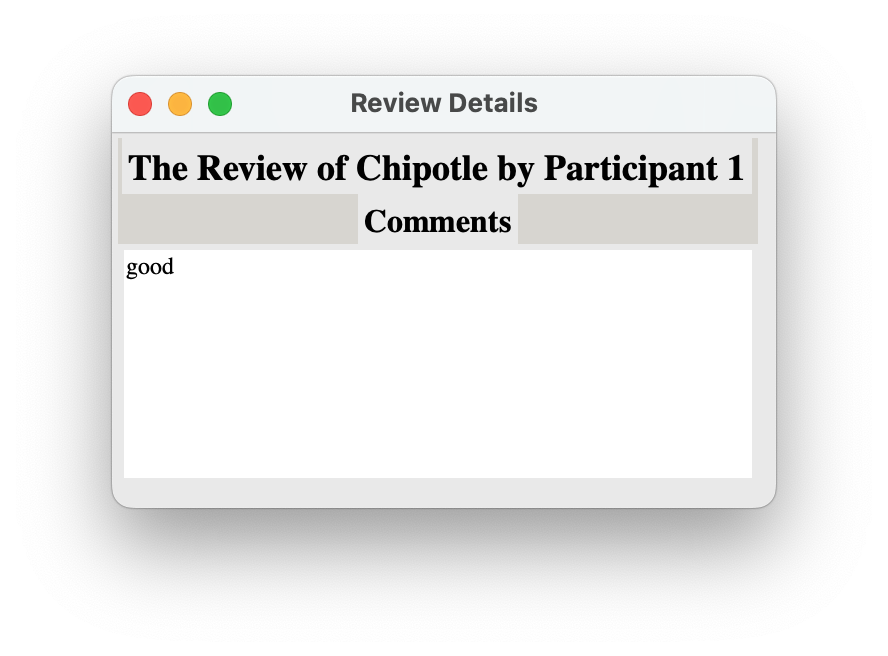
\includegraphics[height=2in]{art/review_details.png}
        \caption{\label{fig:review_details.png}}
    \end{subfigure}
    \caption{Figures for functions on the main canvas.}
\end{figure}

Now we move on to compute the consensus rankings by clicking the ``Compute consensus rankings'' button. 
Since we have both rankings and ratings in the dataset,
we can use all models. We start by selecting the output directory
by using ``Set working directory''.
Then we compute using the default Mallows model, see the result in Figure~\ref{fig:example3}.

  \begin{figure}[h]
    \centering
    \begin{subfigure}[t]{0.5\textwidth}
        \centering
        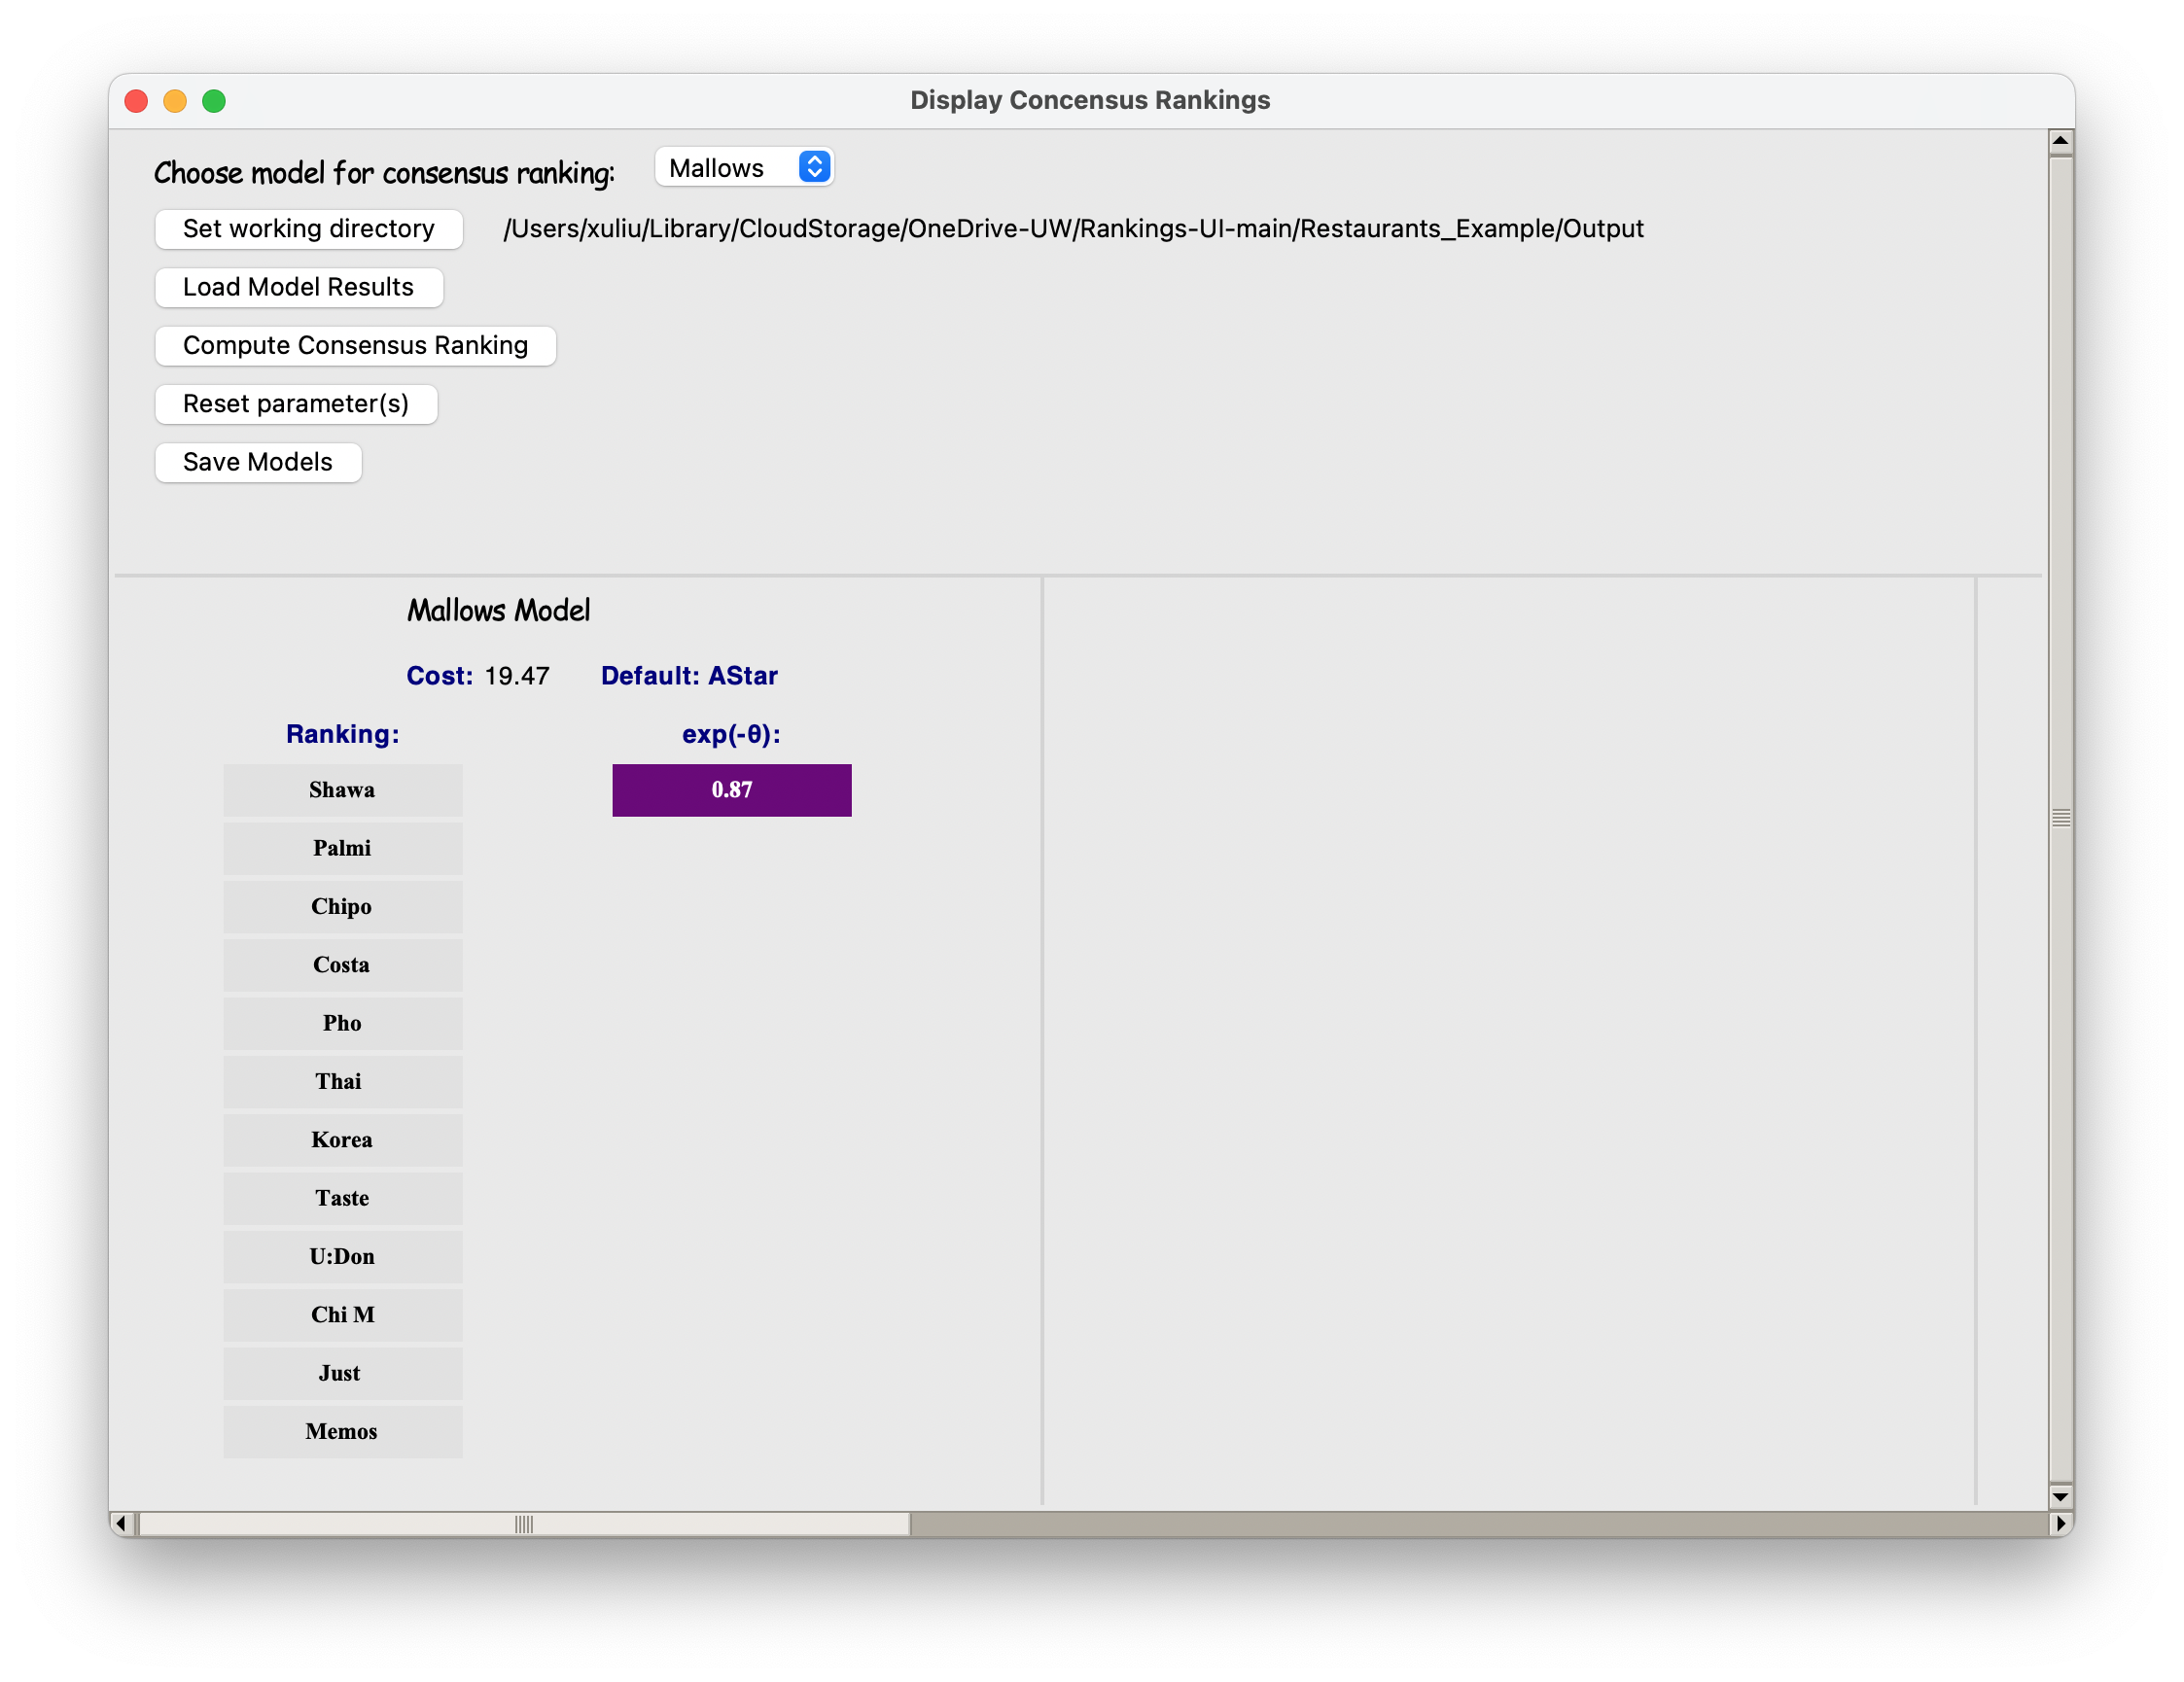
\includegraphics[height=2in]{art/mallows.png}
        \caption{Results from Mallows model.}\label{fig:example3}
    \end{subfigure}%
    ~ 
    \begin{subfigure}[t]{0.5\textwidth}
        \centering
      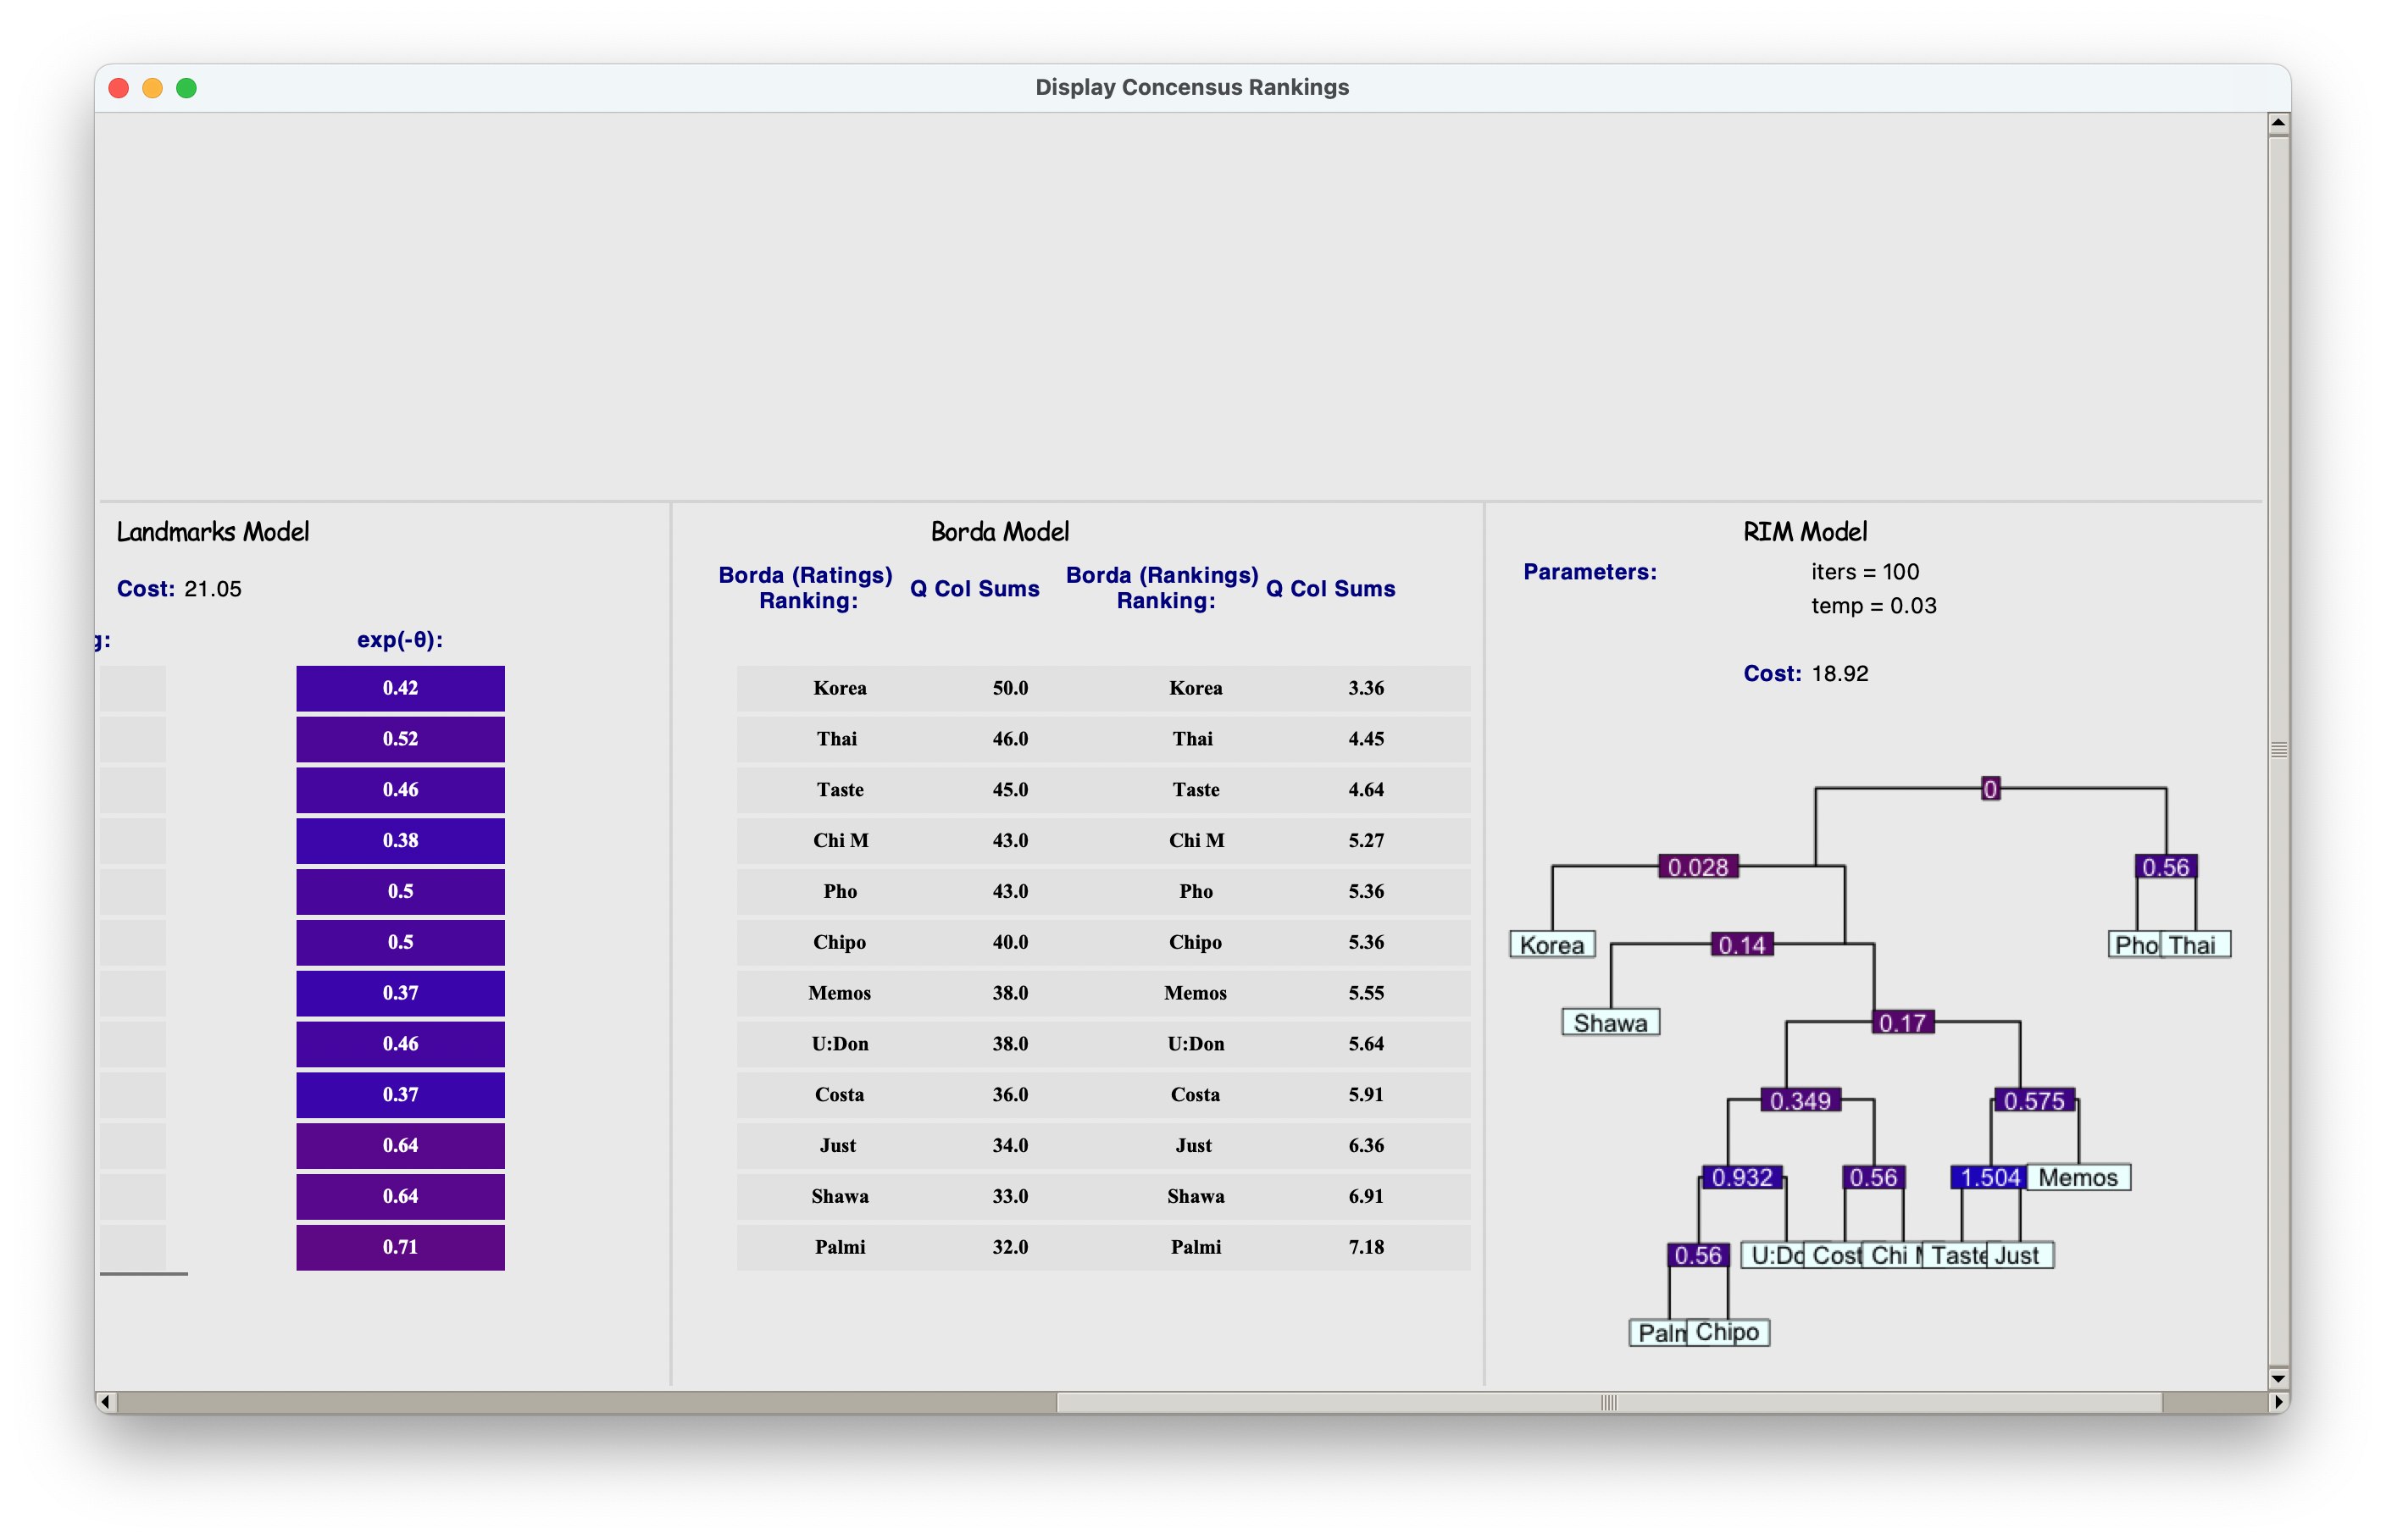
\includegraphics[height=2in]{art/all_models.png}
      \caption{Results from other models.}\label{fig:example4}
    \end{subfigure}
  \end{figure}


Similarly for the rest of the models we can compute them one-by-one, 
see the results in Figure~\ref{fig:example4}.
In the working directory selected, there will be severall folders named by the models,
and each of them will contain the intermediate file(s) from their packages.
We can save the results to a \texttt{.json} file by clicking on the ``Save Models'' button.

Now we move on to compare the models we have
by clicking the ``Performance summary'' button on the main canvas.
We then compare the models with base model Mallows and use
50 bootstrap samples,
see Figure~\ref{fig:summary1} for the settings.

  \begin{figure}[h]
    \begin{center}
      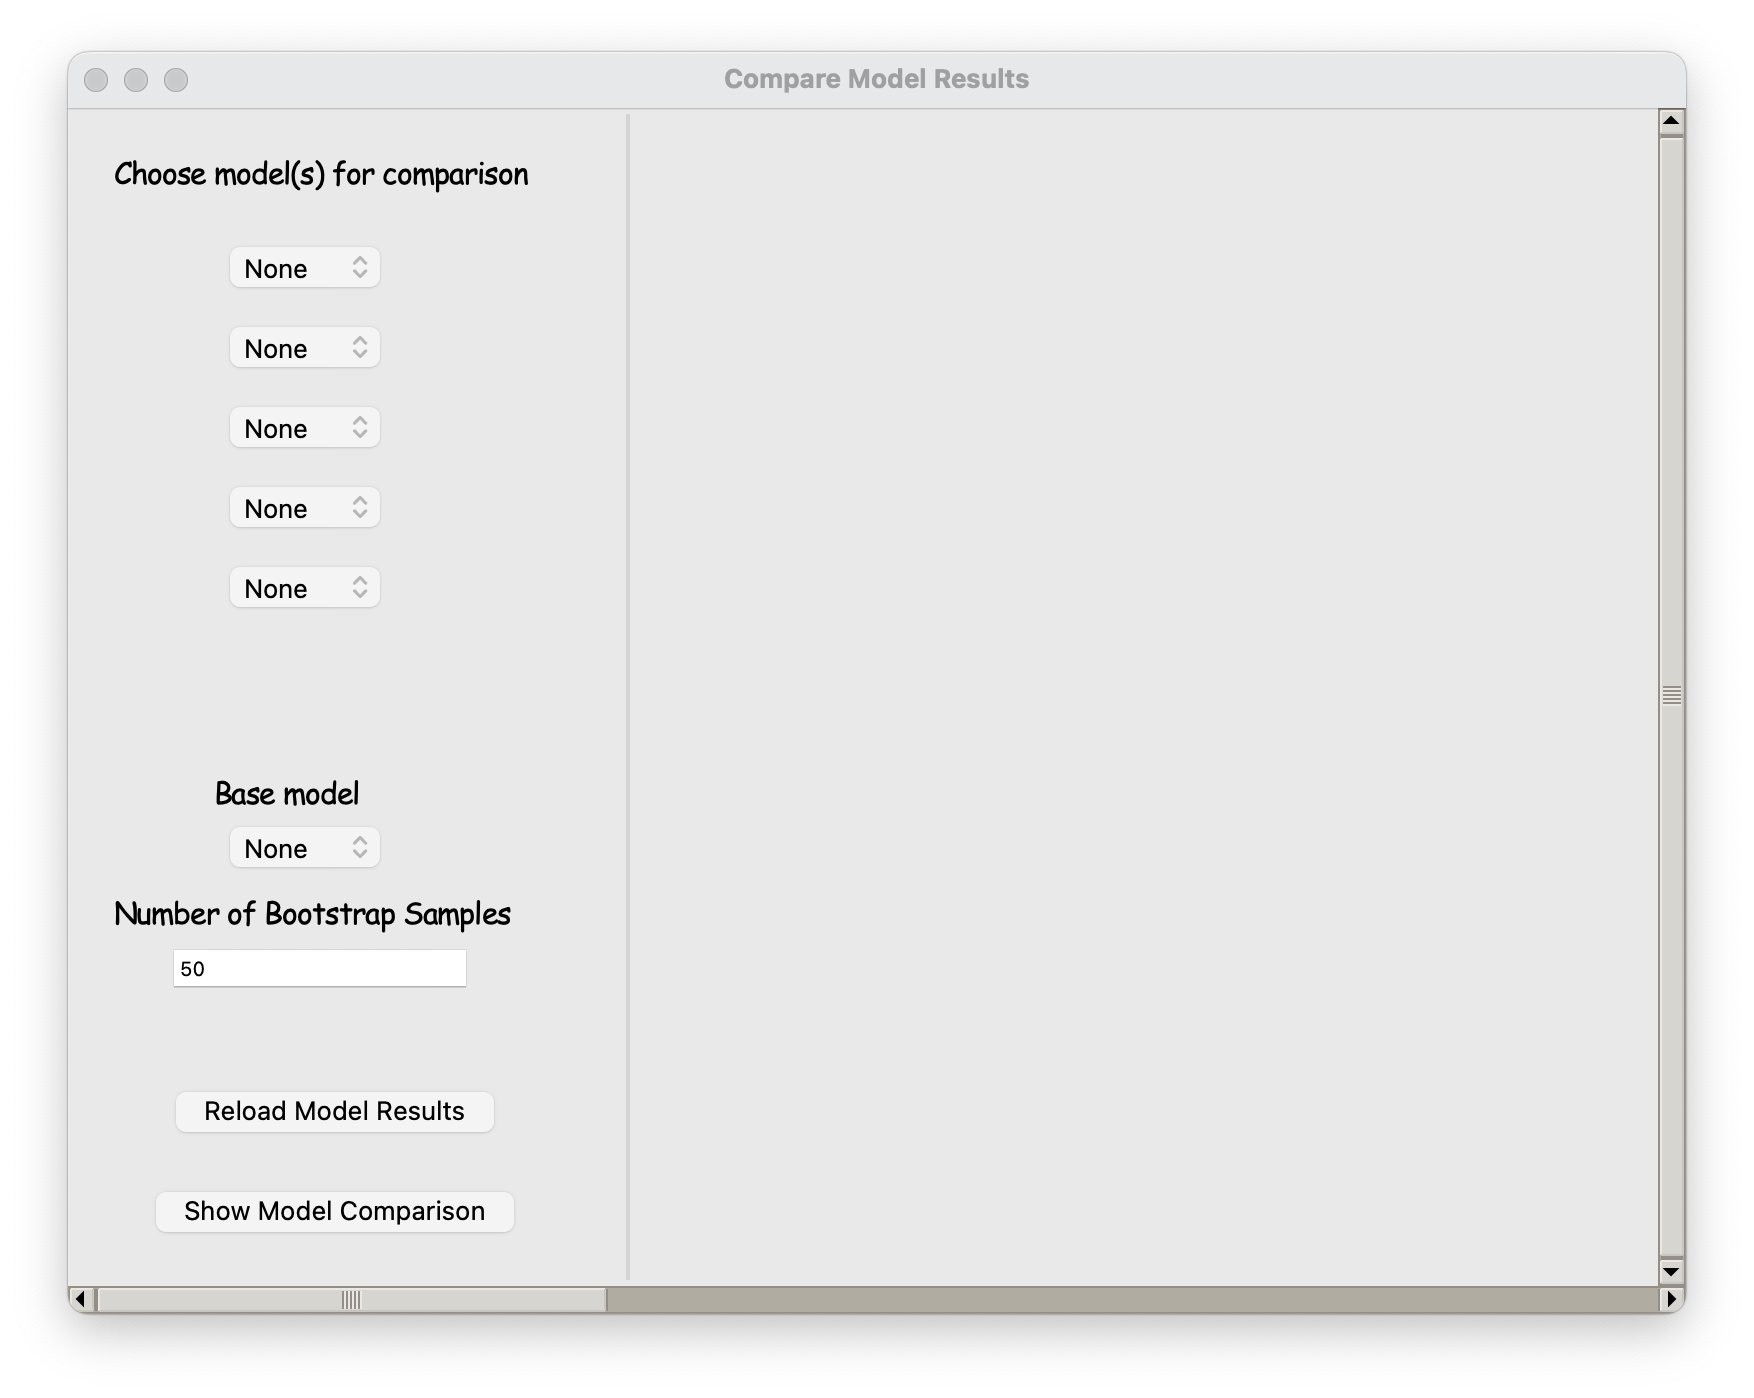
\includegraphics[width=0.6\textwidth]{art/summary_1.png}
      \caption{Loading data into the GUI.}\label{fig:summary1}
    \end{center}
  \end{figure}


  \begin{figure}[h]
    \begin{center}
      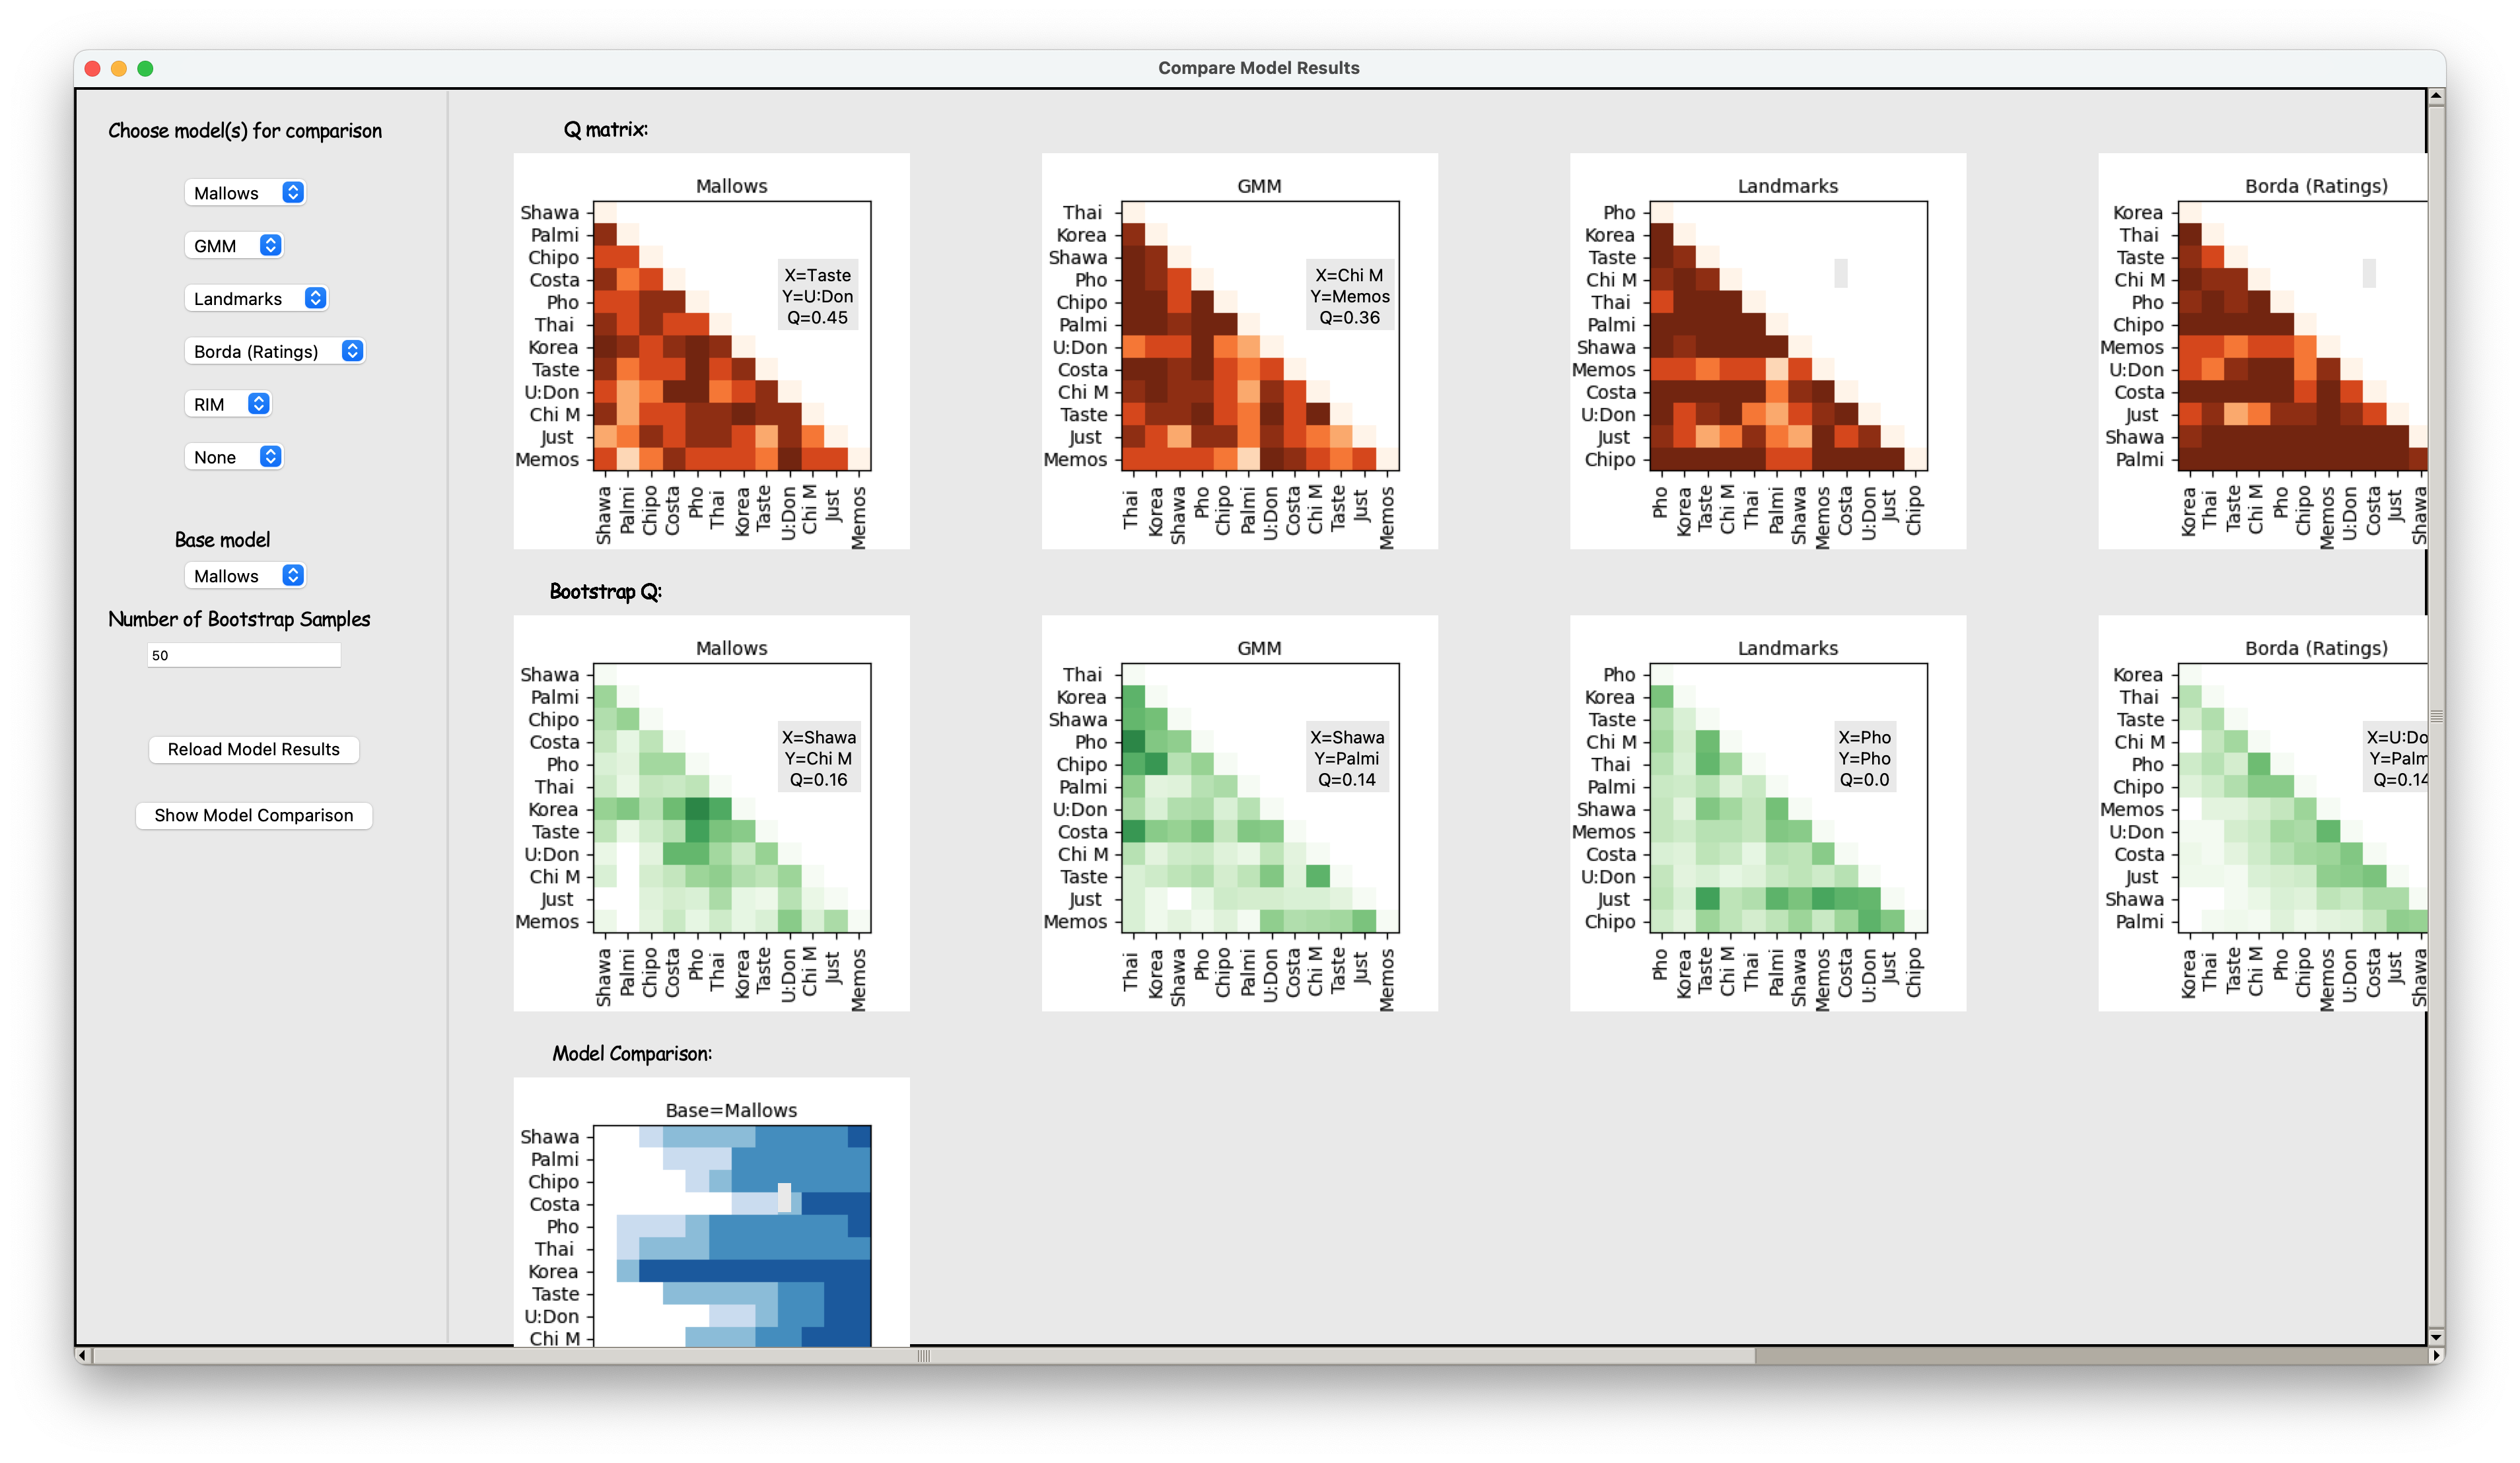
\includegraphics[width=0.95\textwidth]{art/summary_2.png}
      \caption{Loading data into the GUI.}\label{fig:summary2}
    \end{center}
  \end{figure}

The results are in Figure~\ref{fig:summary2}.














\bibliography{ref}

\end{document}